%  Presentación de tesis — Estimación de edad cerebral
%  Beamer 16:9 — tema limpio profesional
\documentclass[aspectratio=169, 11pt]{beamer}

\usepackage[spanish]{babel}
\usepackage[utf8]{inputenc}
\usepackage[T1]{fontenc}

\usetheme{Madrid}
\usecolortheme{default}

\definecolor{uncblue}{RGB}{0, 75, 135}
\definecolor{unclight}{RGB}{220, 235, 250}
\definecolor{uncaccent}{RGB}{200, 60, 50}
\definecolor{uncgray}{RGB}{100, 100, 100}

\setbeamercolor{structure}{fg=uncblue}
\setbeamercolor{palette primary}{bg=uncblue, fg=white}
\setbeamercolor{palette secondary}{bg=uncblue!80, fg=white}
\setbeamercolor{palette tertiary}{bg=uncblue!60, fg=white}
\setbeamercolor{frametitle}{bg=uncblue, fg=white}
\setbeamercolor{title}{fg=uncblue}
\setbeamercolor{block title}{bg=uncblue, fg=white}
\setbeamercolor{block body}{bg=unclight}
\setbeamercolor{block title alerted}{bg=uncaccent, fg=white}
\setbeamercolor{block body alerted}{bg=uncaccent!10}
\setbeamercolor{item}{fg=uncblue}

\setbeamerfont{title}{series=\bfseries, size=\Large}
\setbeamerfont{frametitle}{series=\bfseries}

\setbeamertemplate{navigation symbols}{}
\setbeamertemplate{footline}{%
  \hfill\insertframenumber/\inserttotalframenumber\hspace{4pt}\vspace{2pt}%
}

\usepackage{graphicx}
\graphicspath{{../}}  % figuras en Latex/ (00_tapa, 04_marco_teorico, etc.)
\usepackage{booktabs}
\usepackage{amsmath, amssymb}
\usepackage{tikz}
\usetikzlibrary{arrows.meta, positioning, decorations.pathreplacing}
\usepackage[table]{xcolor}
\usepackage{hyperref}

\newcommand{\highlight}[1]{\textcolor{uncaccent}{\textbf{#1}}}
\newcommand{\bref}[1]{\textcolor{uncgray}{\scriptsize [#1]}}

\title{Estimación de la edad cerebral mediante autoencoders variacionales y aprendizaje multimodal a partir de conectividad funcional, datos estructurales y variables sociodemográficas}
\author{Nicolás Marcelo Bazán}
\institute{%
  Facultad de Matemática, Astronomía, Física y Computación\\
  Universidad Nacional de Córdoba\\[6pt]
  
\includegraphics[height=1cm]{00_tapa/figures/logo_famaf.png}
  \hspace{1cm}
  
\includegraphics[height=1cm]{00_tapa/figures/logo_unc.png}
}
\date{2026}

\begin{document}

\begin{frame}[plain]
  \vfill
  \centering
  {\usebeamerfont{title}\color{uncblue}\inserttitle\par}
  \vspace{0.35cm}
  {\usebeamerfont{subtitle}\color{black!80}\insertsubtitle\par}
  \vspace{0.55cm}
  {\usebeamerfont{author}\insertauthor\par}
  \vspace{0.2cm}
  {\usebeamerfont{institute}\insertinstitute\par}
  \vspace{0.35cm}
  {\usebeamerfont{date}\insertdate\par}
  \vfill
\end{frame}

\begin{frame}{Estructura de la presentación}
  \tableofcontents
\end{frame}


\section{Motivación}

\begin{frame}{El cerebro envejece}
  \begin{columns}[T]
    \begin{column}{0.55\textwidth}
      \begin{itemize}
        \item El cerebro cambia con la edad de forma gradual y predecible
        \item Se pierde volumen de \highlight{materia gris}, se adelgaza la corteza
        \item Cambian los patrones de \highlight{conectividad} entre regiones
        \item Enfermedades como el Alzheimer o la demencia frontotemporal \textbf{aceleran} este proceso
      \end{itemize}
    \end{column}
    \begin{column}{0.42\textwidth}
      \centering
      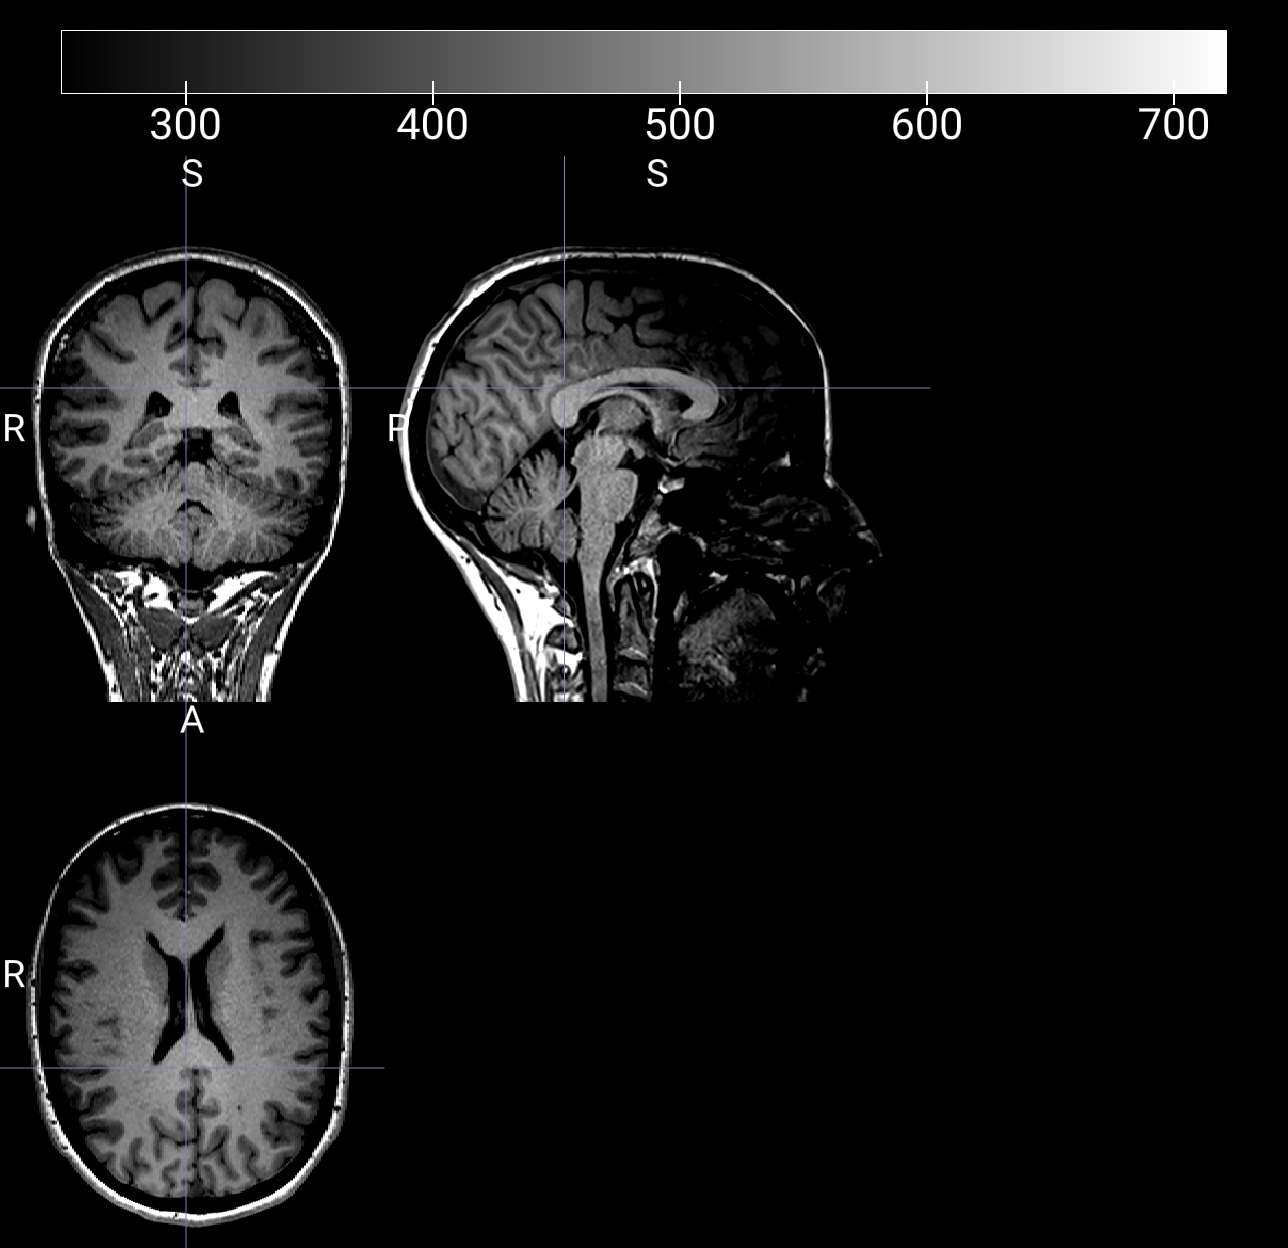
\includegraphics[width=\textwidth]{04_marco_teorico/images/t1_structural.png}\\[4pt]
      {\scriptsize Imagen T1w de resonancia magnética}
    \end{column}
  \end{columns}
\end{frame}

\begin{frame}{Brain Age Gap: la idea central}
  \centering
  \shorthandoff{>}
  \begin{tikzpicture}[
    box/.style={draw, rounded corners, text width=3cm, align=center,
                minimum height=1cm, font=\small},
    arr/.style={-{Stealth[length=3mm]}, thick, uncblue}
  ]
    \node[box, fill=unclight] (img) {Imagen cerebral\\del sujeto};
    \node[box, fill=unclight, right=1.8cm of img] (model) {Modelo\\predictivo};
    \node[box, fill=unclight, right=1.8cm of model] (pred) {Edad predicha\\$\hat{y} = 72$ años};
    \draw[arr] (img) -- (model);
    \draw[arr] (model) -- (pred);
  \end{tikzpicture}
  \shorthandon{>}

  \vspace{0.4cm}
  \begin{columns}[T]
    \begin{column}{0.46\textwidth}
      \begin{block}{Si la edad real es 65}
        \centering
        Gap $= 72 - 65 = \highlight{+7}$\\[3pt]
        {\small Envejecimiento \textbf{acelerado}}
      \end{block}
    \end{column}
    \begin{column}{0.46\textwidth}
      \begin{block}{Si la edad real es 78}
        \centering
        Gap $= 72 - 78 = \textcolor{green!50!black}{\textbf{-6}}$\\[3pt]
        {\small Cerebro ``más joven''}
      \end{block}
    \end{column}
  \end{columns}

  \vspace{0.3cm}
  {\small \textbf{Objetivo de este trabajo:} 
  \begin{itemize}
    \item Predecir la edad cerebral
    \item Analizar qué variables demográficas modulan esta predicción
    \item Explorar la viabilidad como biomarcador de envejecimiento acelerado
  \end{itemize}
  }
\end{frame}


\section{Marco teórico}

\begin{frame}{Resonancia magnética (MRI)}
  \begin{columns}[T]
    \begin{column}{0.55\textwidth}
      \begin{itemize}
        \item Técnica \textbf{no invasiva} basada en campos magnéticos y pulsos electromagnéticos
        \item Según la secuencia de pulsos utilizada, se obtienen \textbf{distintos contrastes} entre tejidos
        \item Las imágenes están compuestas por \highlight{vóxeles}: la extensión 3D del píxel
        \item Las imágenes \textbf{T1w} (T1-weighted) distinguen claramente materia gris, materia blanca y líquido cefalorraquídeo
      \end{itemize}

      \vspace{0.15cm}
      {\small La \highlight{materia gris} contiene los cuerpos neuronales; su volumen \textbf{disminuye con la edad}.}
    \end{column}
    \begin{column}{0.42\textwidth}
      \centering
      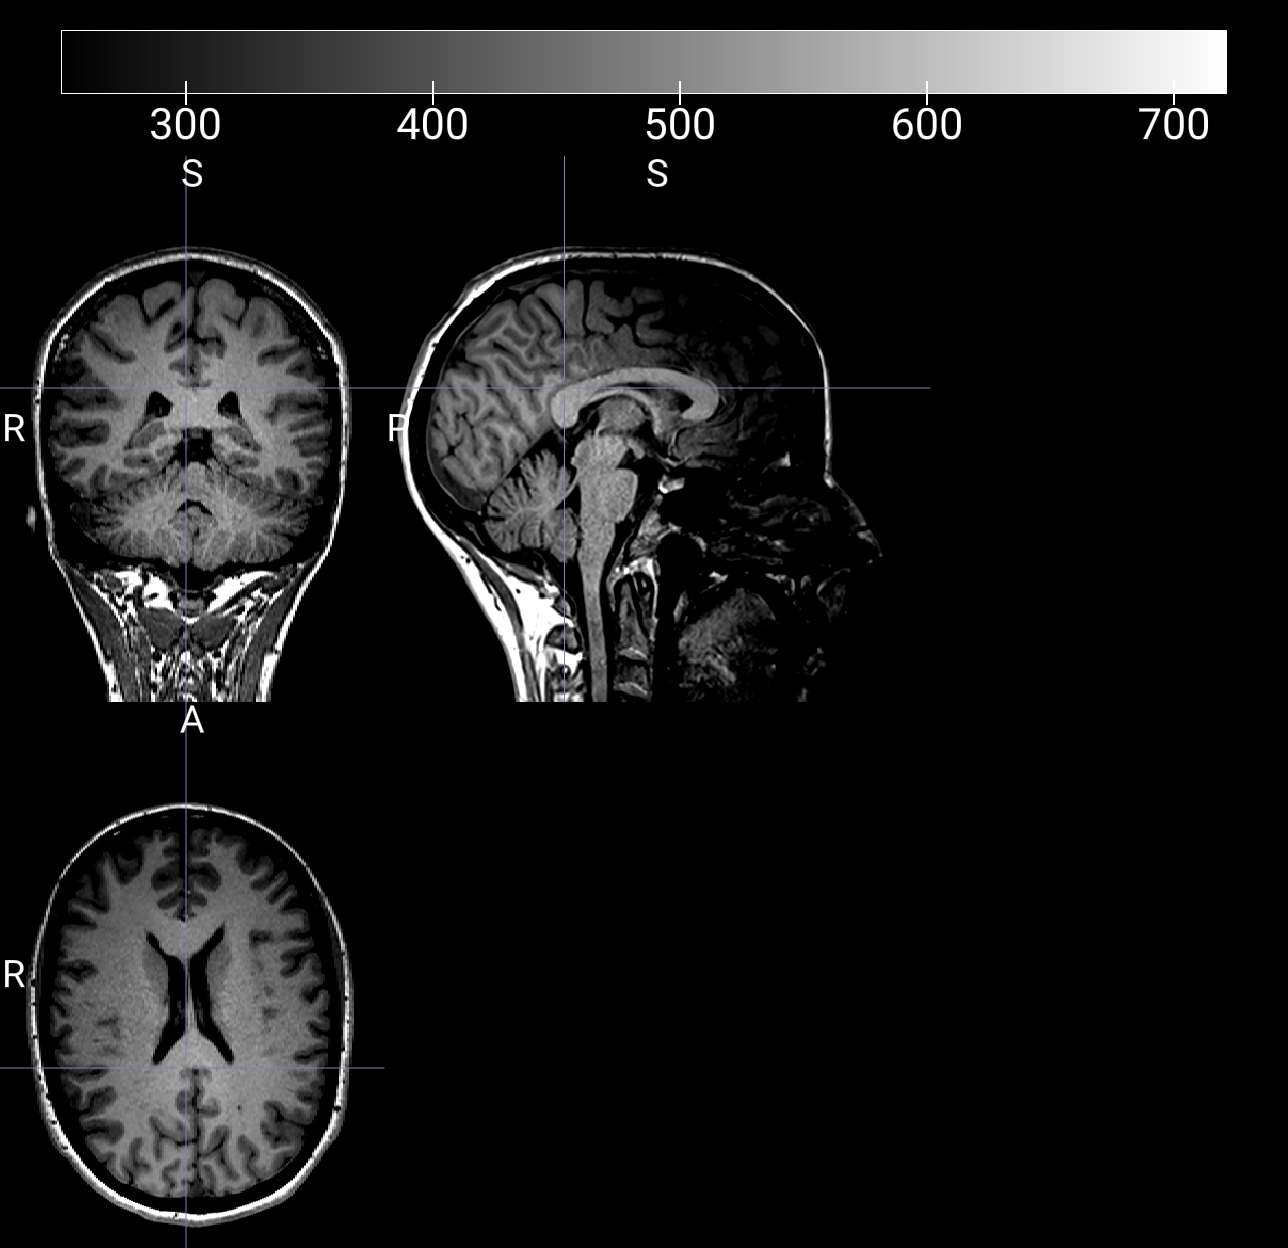
\includegraphics[width=\textwidth]{04_marco_teorico/images/t1_structural.png}\\[4pt]
      {\scriptsize Imagen T1w de un sujeto.\\Referencia anatómica del cerebro.}
    \end{column}
  \end{columns}
\end{frame}

\begin{frame}{Espacio estándar y parcelación cerebral}
  \begin{columns}[T]
    \begin{column}{0.50\textwidth}
      \begin{itemize}
        \item Los cerebros difieren en forma y tamaño $\rightarrow$ se necesita un \textbf{espacio de referencia común}
        \item La plantilla \highlight{MNI152} se construye promediando imágenes de muchos sujetos
        \item Cada cerebro se alinea a este espacio mediante transformaciones espaciales
        \item El \highlight{atlas AAL} divide el cerebro estándar en \textbf{116 regiones} anatómicas
      \end{itemize}

      \vspace{0.1cm}
      {\small En este trabajo: \textbf{116 volúmenes regionales} de materia gris por sujeto (atlas AAL).}
    \end{column}
    \begin{column}{0.47\textwidth}
      \centering
      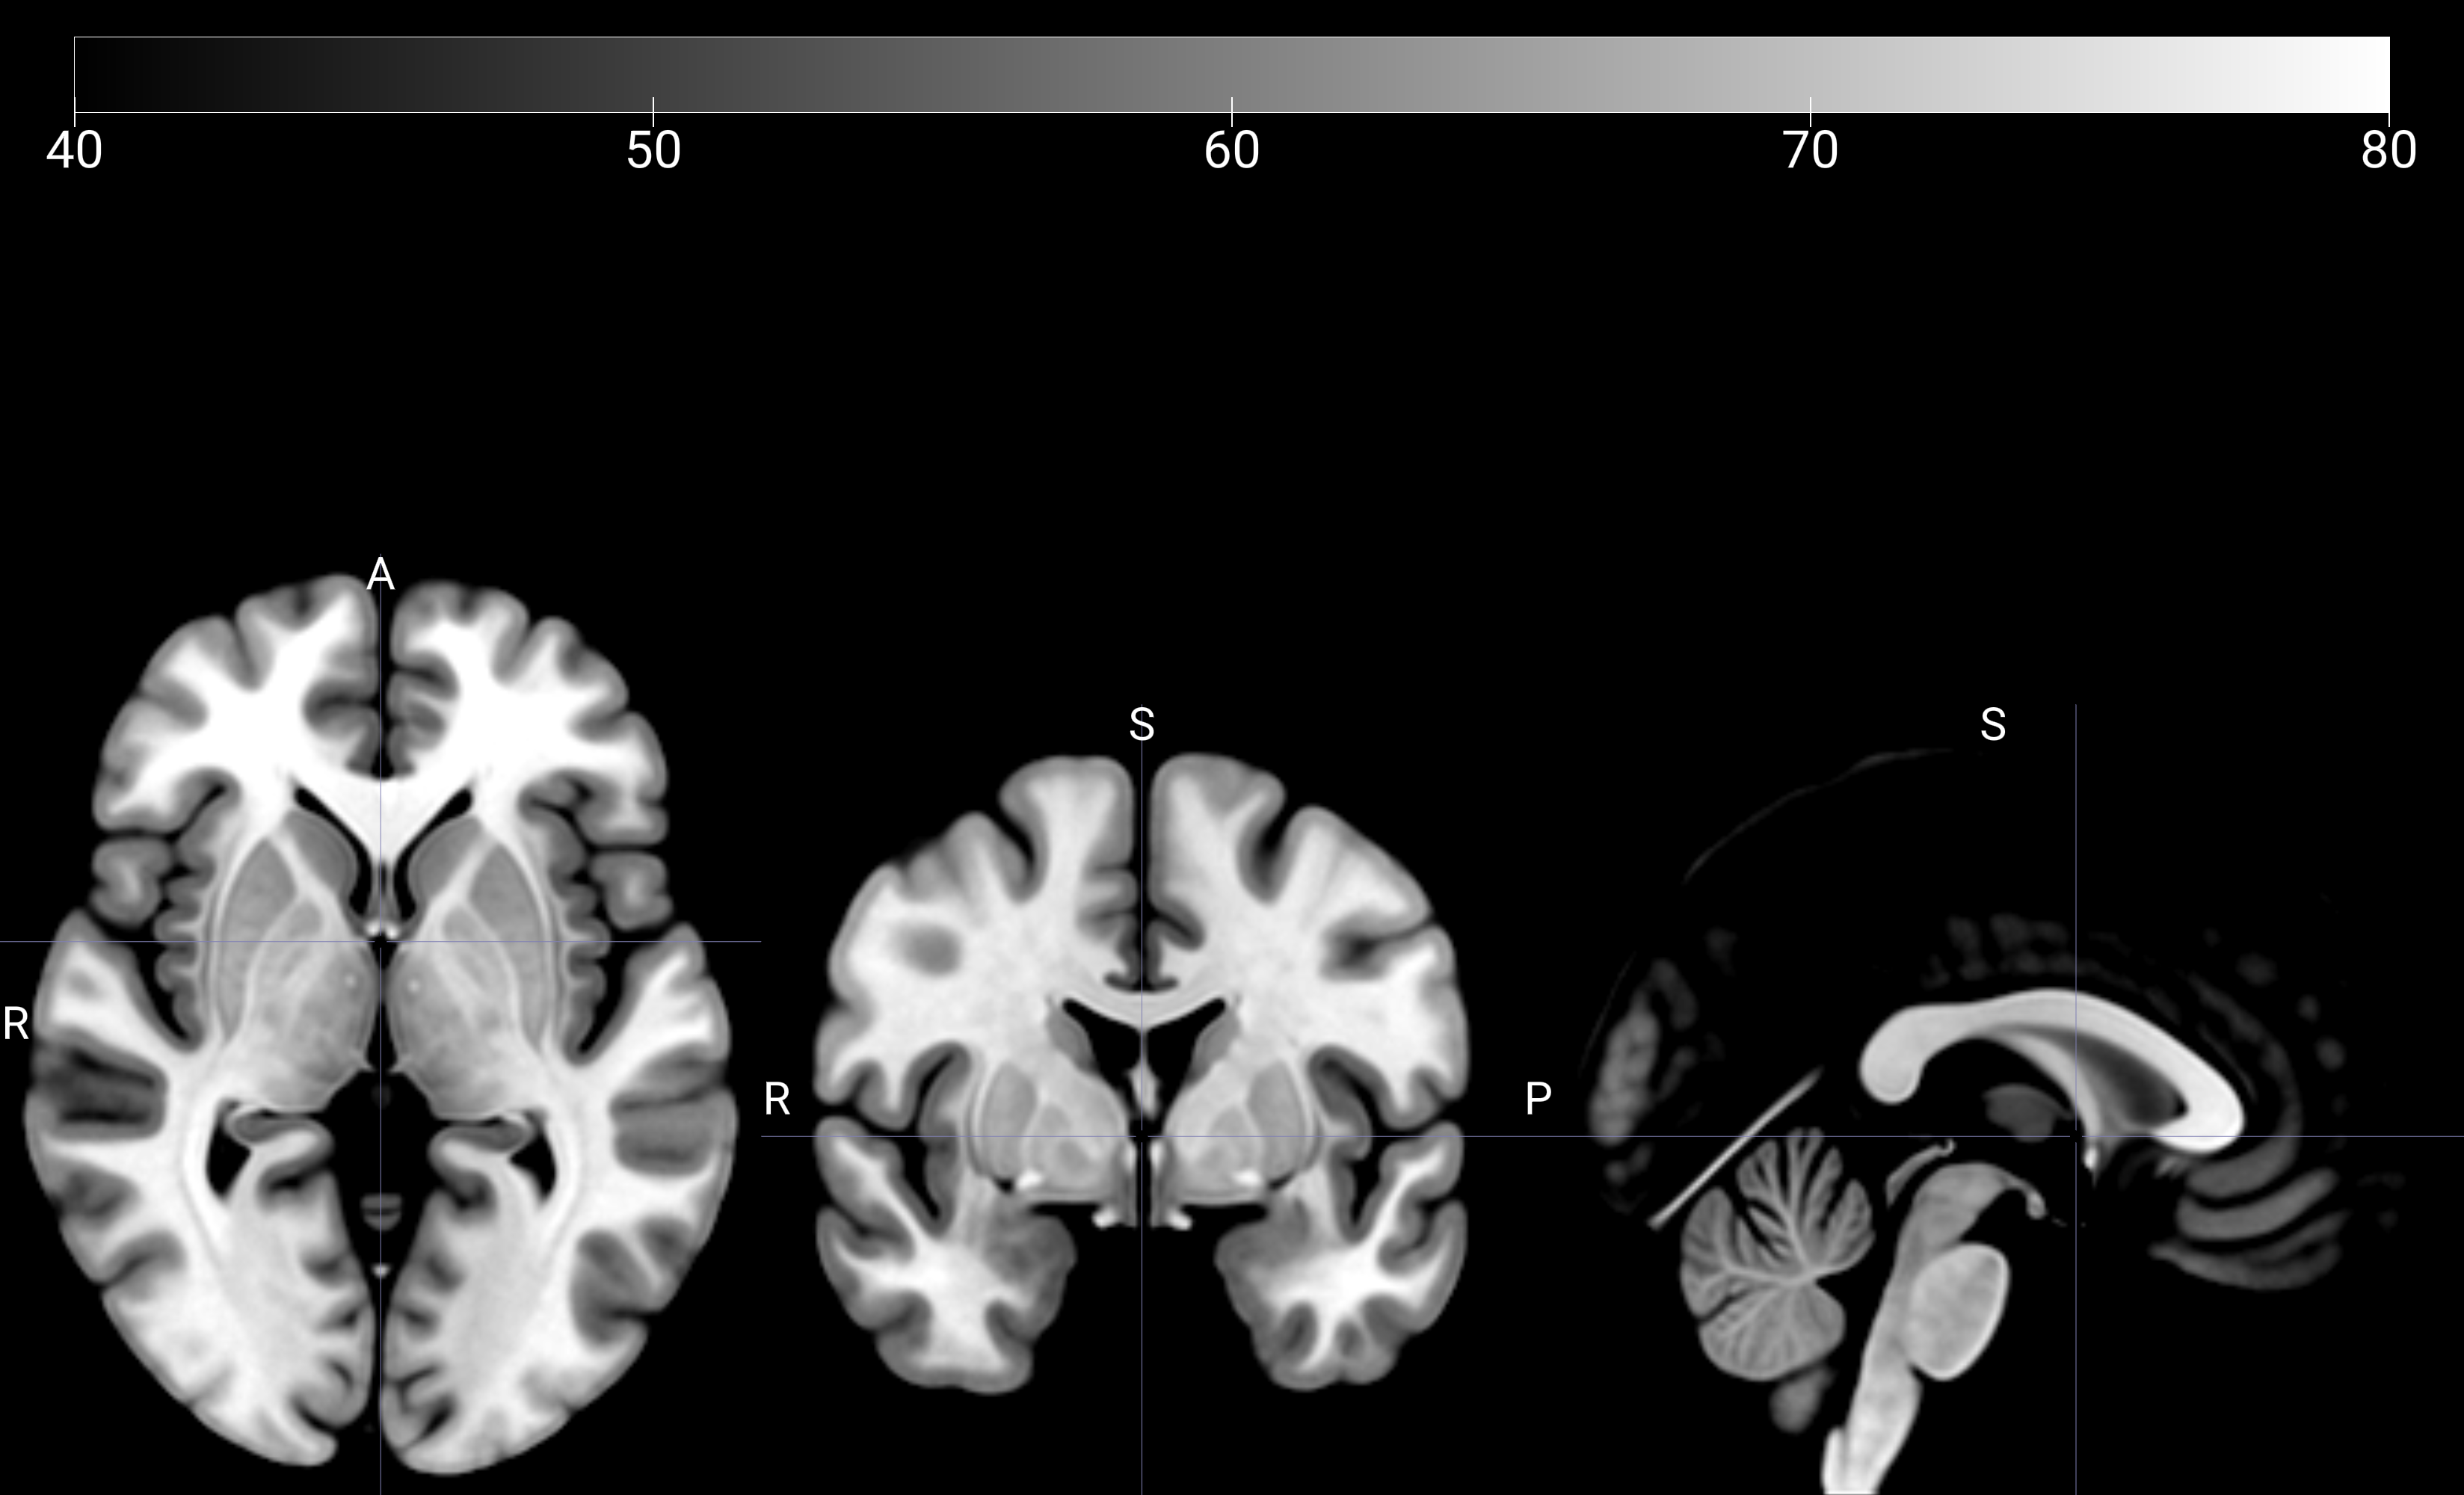
\includegraphics[width=0.72\textwidth]{04_marco_teorico/images/mni152.png}\\[1pt]
      {\scriptsize Plantilla MNI152}\\[3pt]
      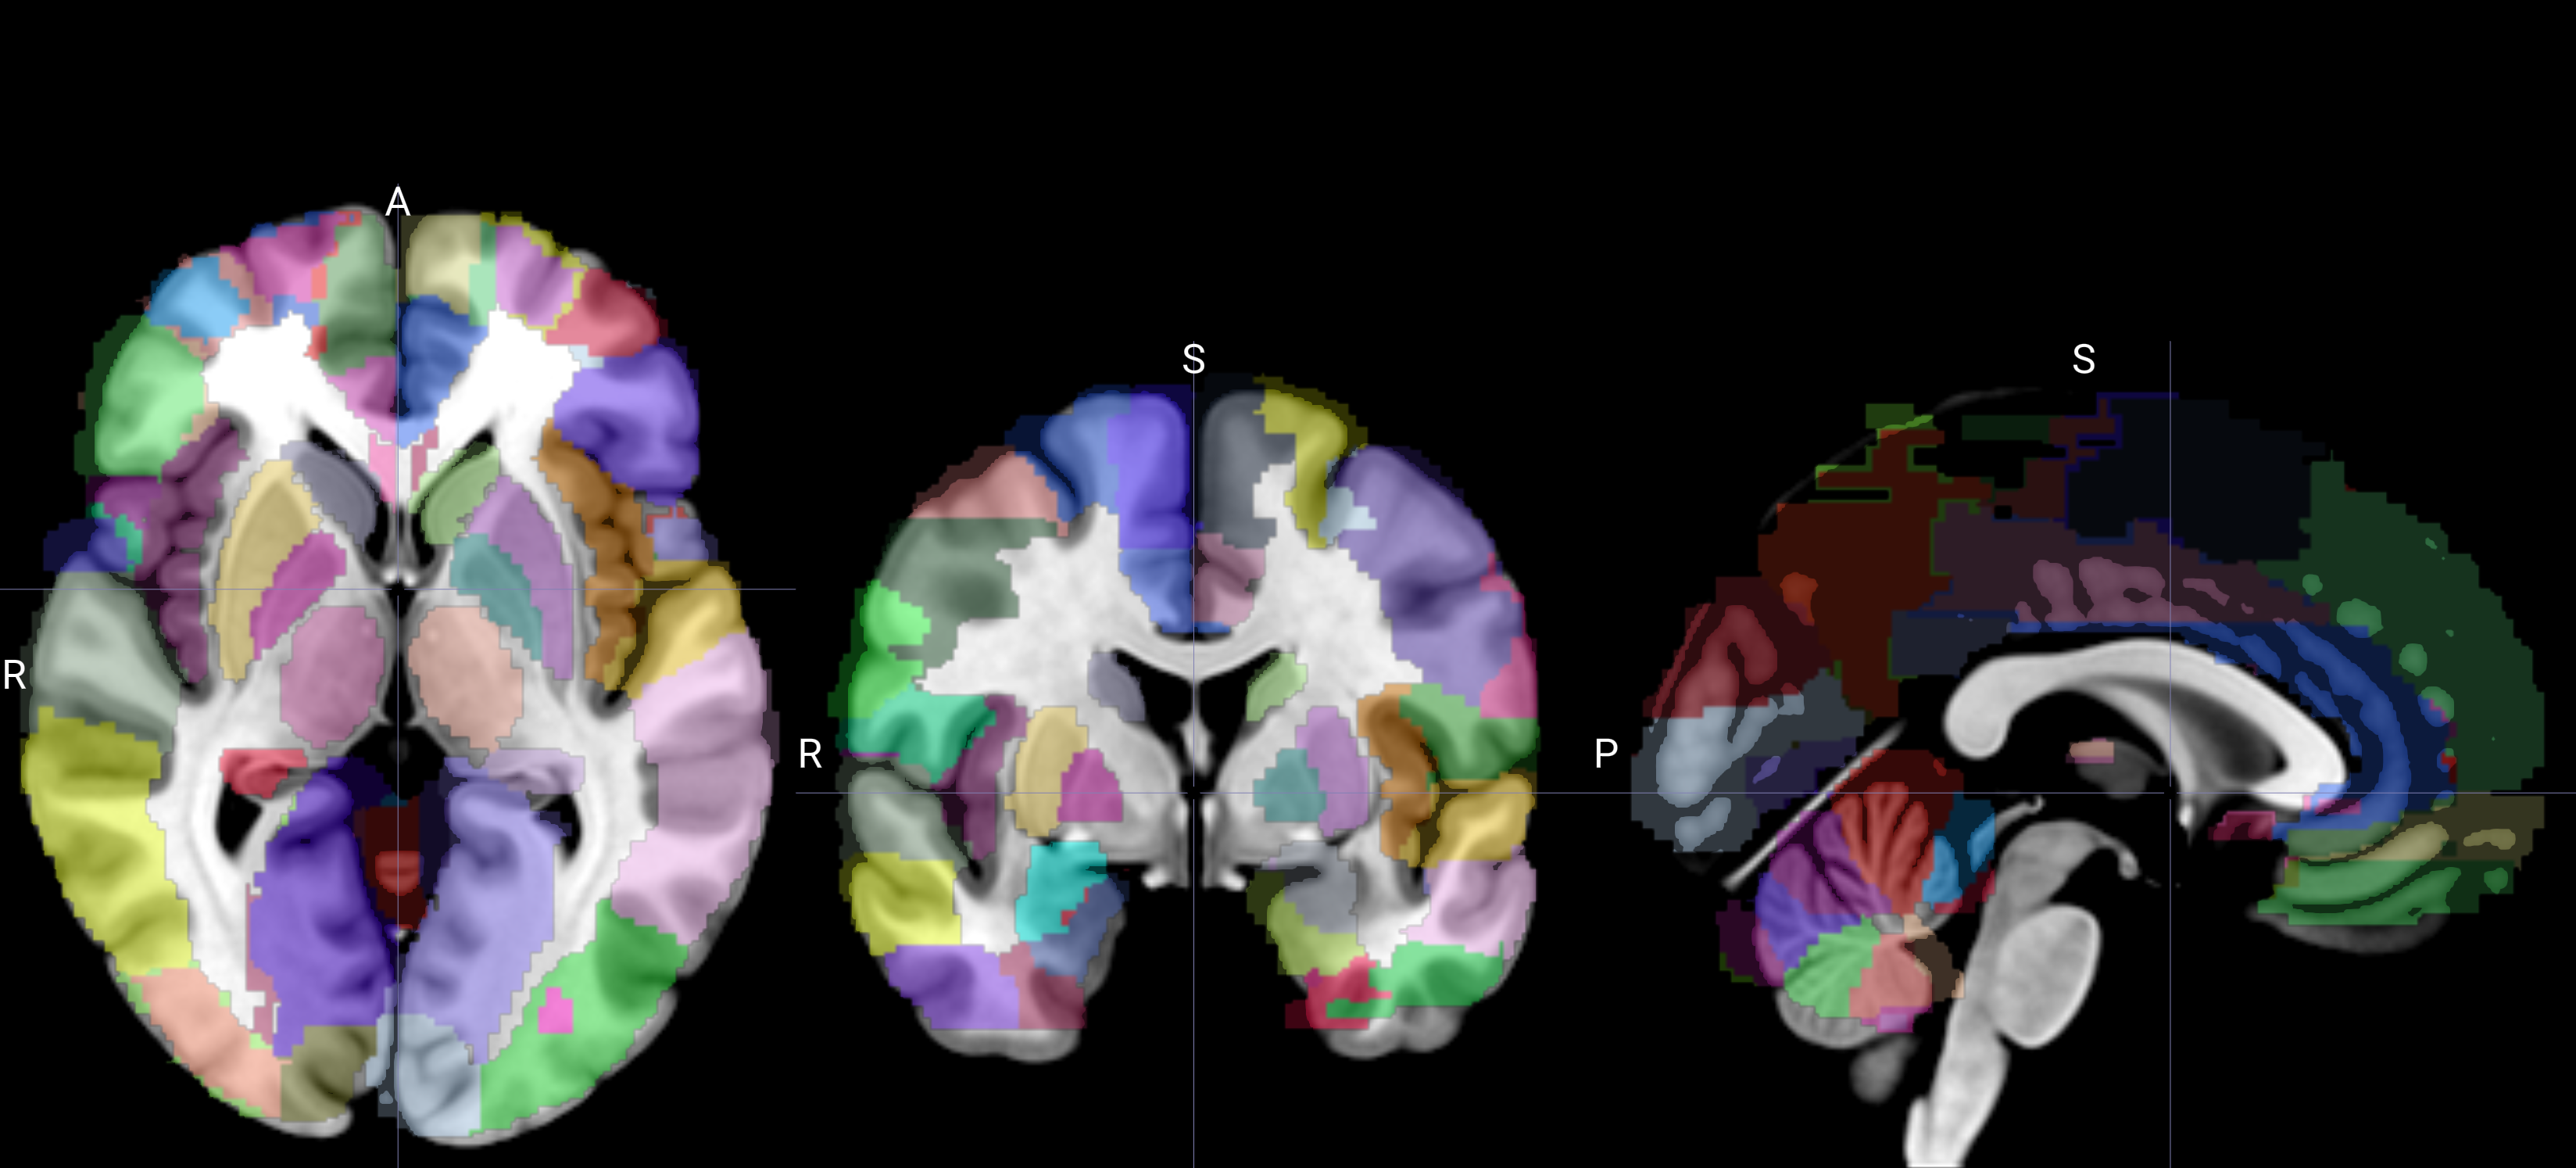
\includegraphics[width=0.72\textwidth]{04_marco_teorico/images/mni152+atlas.png}\\[1pt]
      {\scriptsize Atlas AAL superpuesto.\\Cada color = una región.}
    \end{column}
  \end{columns}
\end{frame}

\begin{frame}{fMRI en reposo y señal BOLD}
  \begin{columns}[T]
    \begin{column}{0.50\textwidth}
      \begin{itemize}
        \item El \highlight{fMRI} mide la actividad cerebral de forma indirecta
        \item Detecta cambios en el flujo sanguíneo (\textbf{señal BOLD})
        \item En ``reposo'': el sujeto no realiza ninguna tarea
        \item Se obtiene una serie temporal por cada región cerebral
      \end{itemize}

      \vspace{0.2cm}
      {\small Regiones que fluctúan de forma sincronizada $\rightarrow$ están \textbf{funcionalmente conectadas}}
    \end{column}
    \begin{column}{0.47\textwidth}
      \centering
      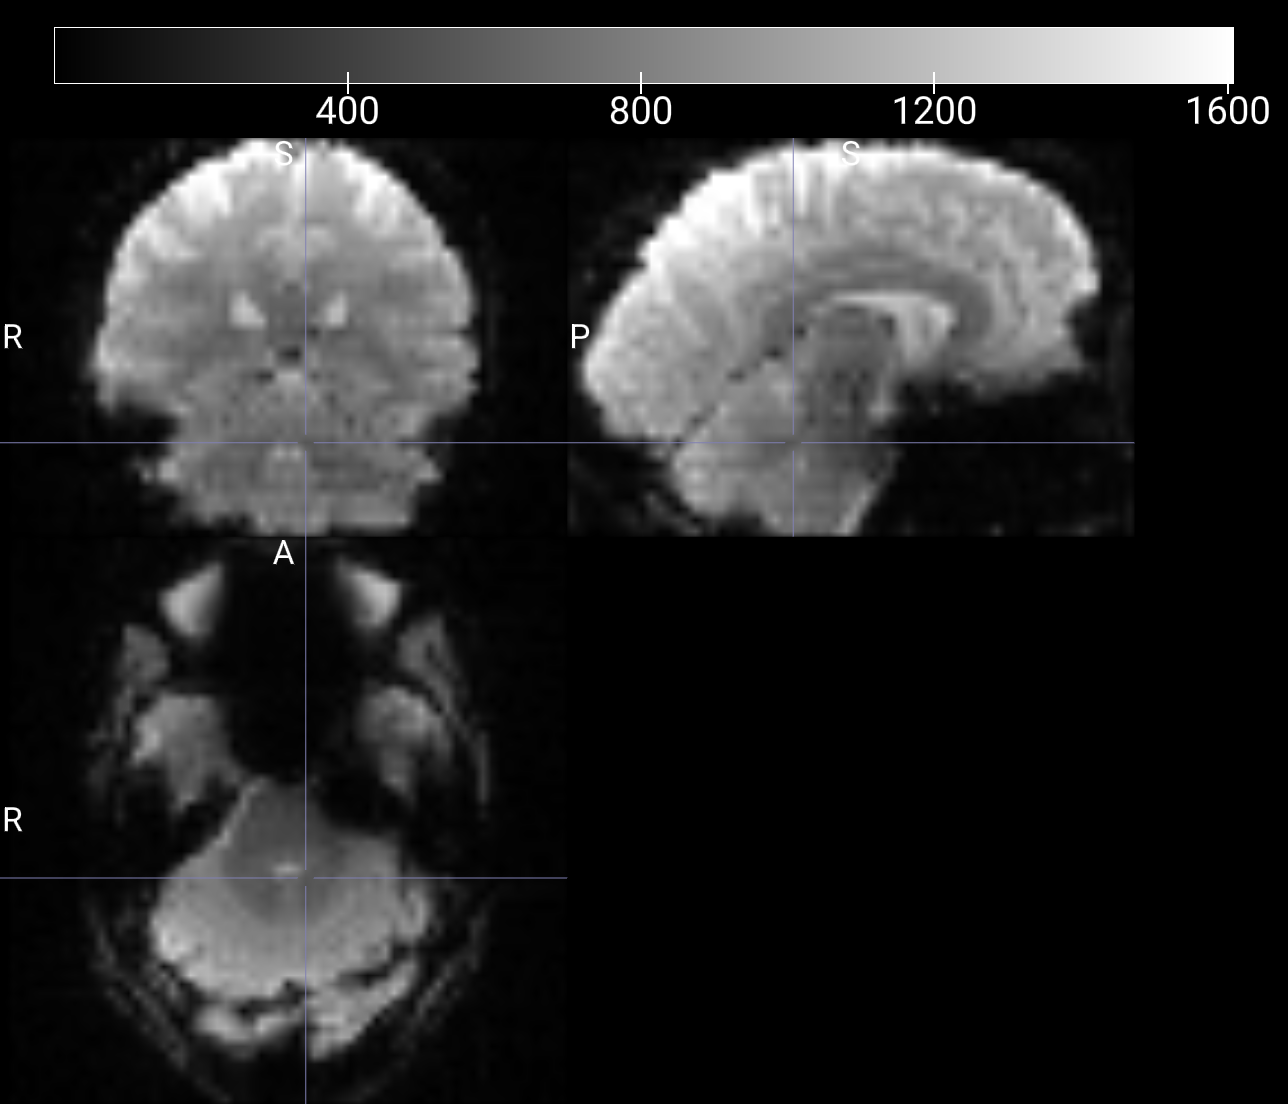
\includegraphics[width=0.80\textwidth]{04_marco_teorico/images/bold_volume.png}\\[2pt]
      {\scriptsize Volumen cerebral captado por fMRI}\\[5pt]
      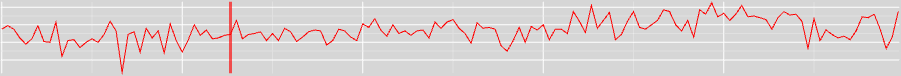
\includegraphics[width=0.95\textwidth]{04_marco_teorico/images/bold_timeseries.png}\\[2pt]
      {\scriptsize Serie temporal BOLD de una región}
    \end{column}
  \end{columns}
\end{frame}

\begin{frame}{Conectividad funcional}
  \begin{columns}[T]
    \begin{column}{0.50\textwidth}
      \centering
      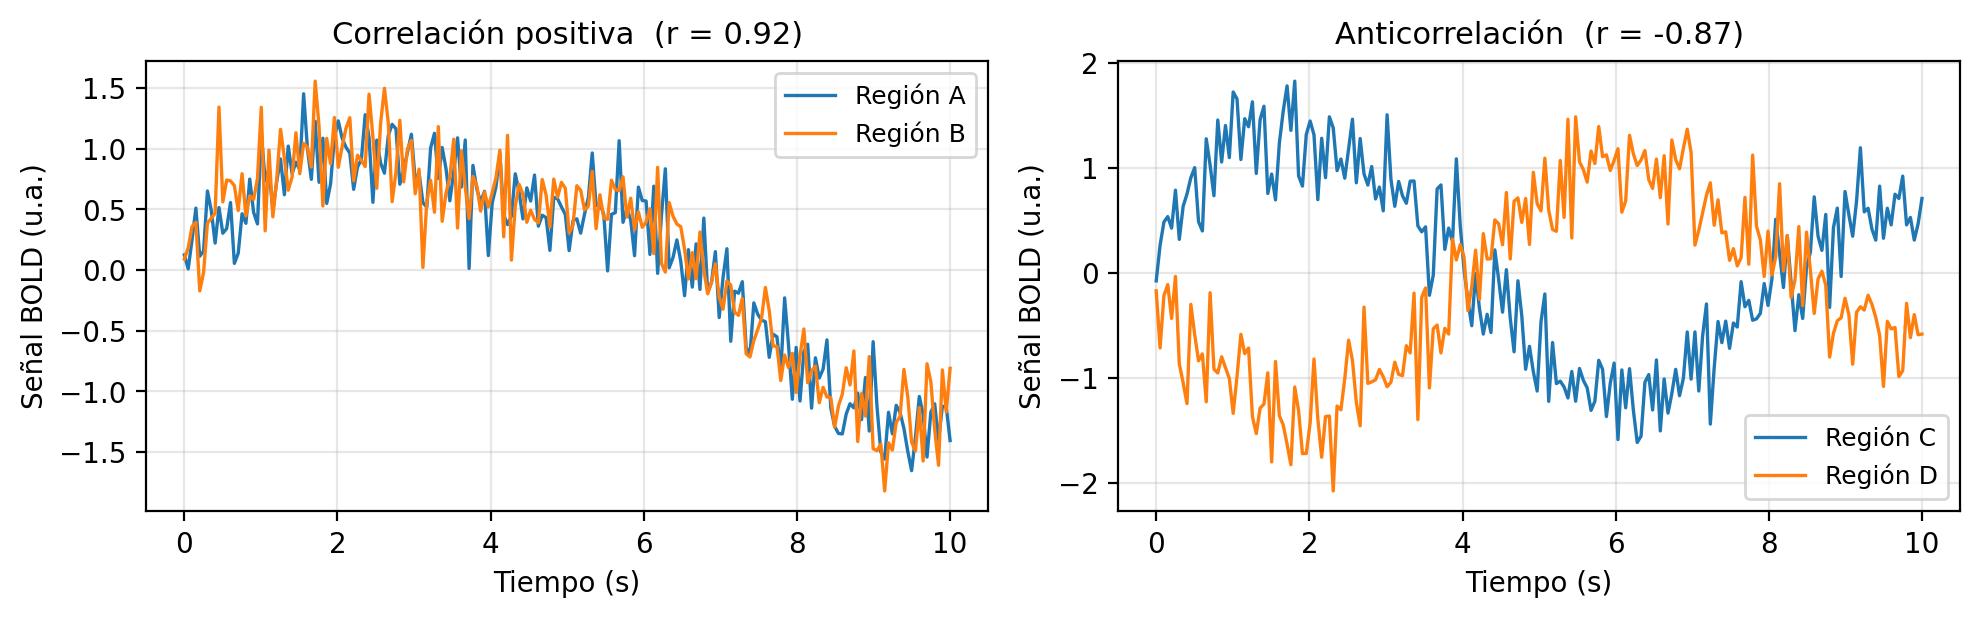
\includegraphics[width=0.92\textwidth]{04_marco_teorico/images/timeseries_correlation.png}\\[2pt]
      {\scriptsize Correlación positiva ($r = 0{,}92$) y anticorrelación ($r = -0{,}87$) entre pares de regiones}

      \vspace{0.1cm}
      \begin{itemize}
        \item Se calcula la \highlight{correlación de Pearson} entre cada par de regiones
        \item Resultado: matriz simétrica $116 \times 116$
        \item Triángulo superior: \highlight{6670 valores} por sujeto
      \end{itemize}
    \end{column}
    \begin{column}{0.47\textwidth}
      \centering
      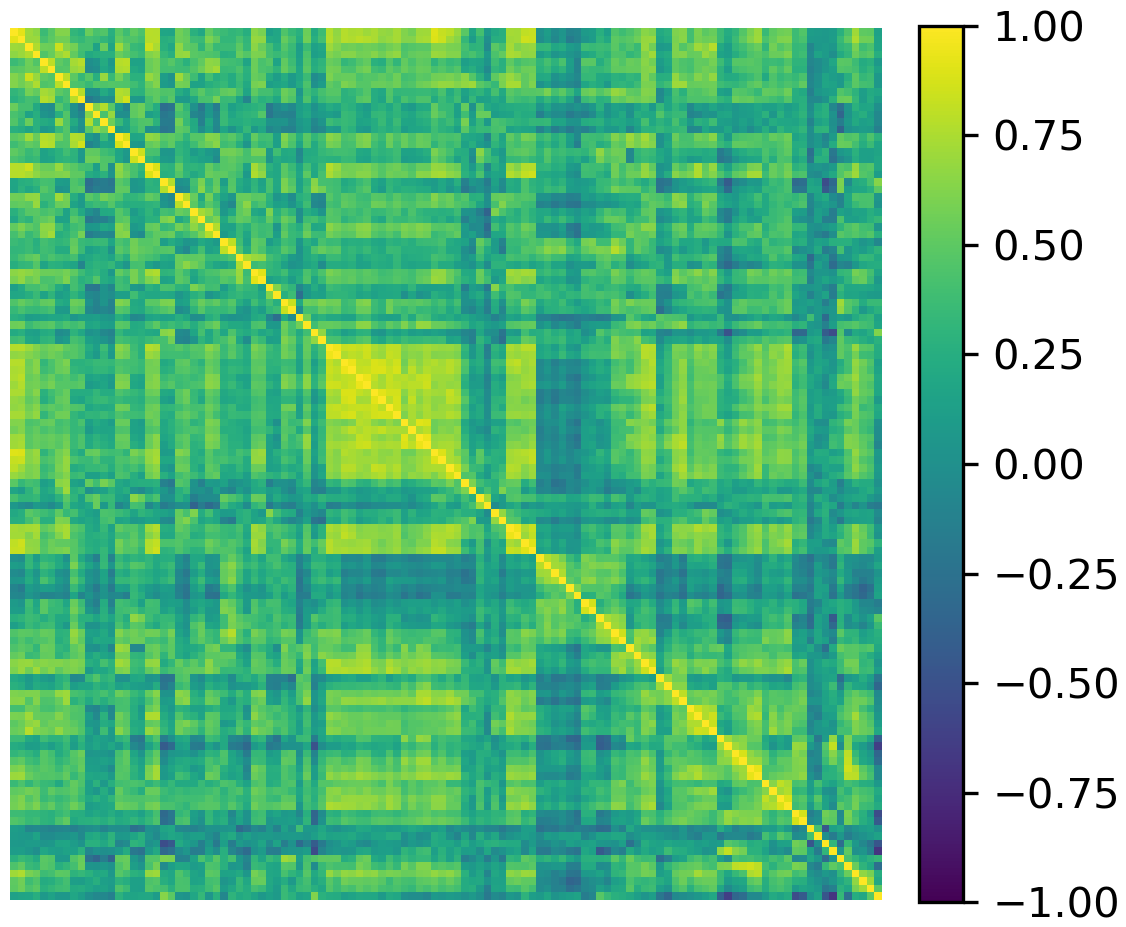
\includegraphics[width=0.85\textwidth]{04_marco_teorico/images/fc_example.png}\\[2pt]
      {\scriptsize Matriz de conectividad funcional\\$116 \times 116$ (atlas AAL)}
    \end{column}
  \end{columns}
\end{frame}

\begin{frame}{El desafío: alta dimensionalidad}
  \begin{alertblock}{Problema ``small-n, large-p''}
    6670 features de conectividad funcional, pero solo $N = 1245$ sujetos $\rightarrow$ riesgo de \textbf{sobreajuste}.
  \end{alertblock}

  \vspace{0.1cm}
  \begin{columns}[T]
    \begin{column}{0.46\textwidth}
      \centering
      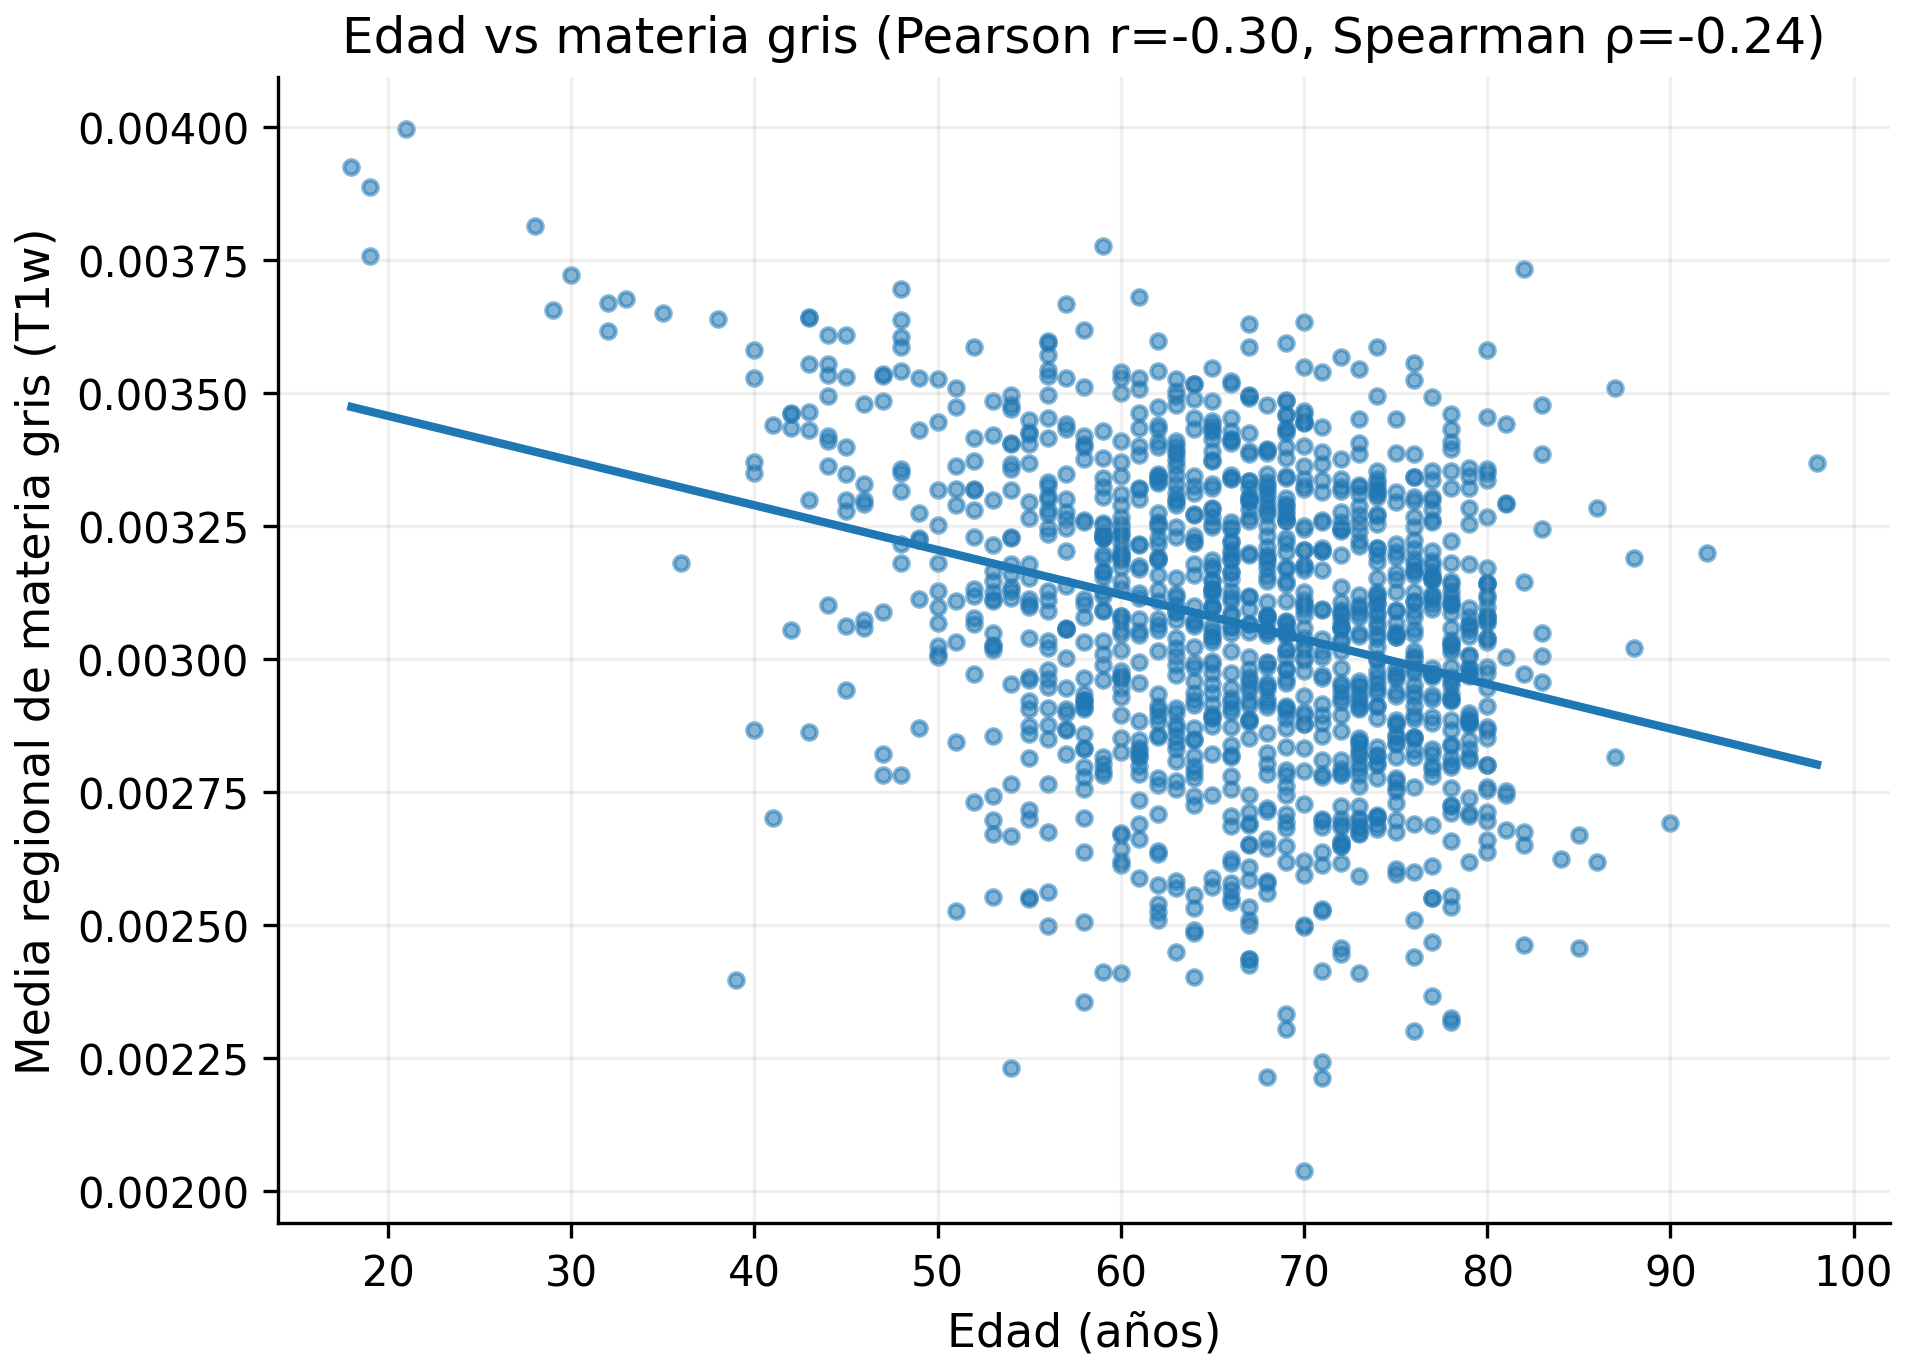
\includegraphics[width=0.80\textwidth]{05_datos_cohorte/images/corr_age_gmmean.png}\\[2pt]
      {\scriptsize Materia gris vs.\ edad: $r = -0{,}30$}
    \end{column}
    \begin{column}{0.46\textwidth}
      \centering
      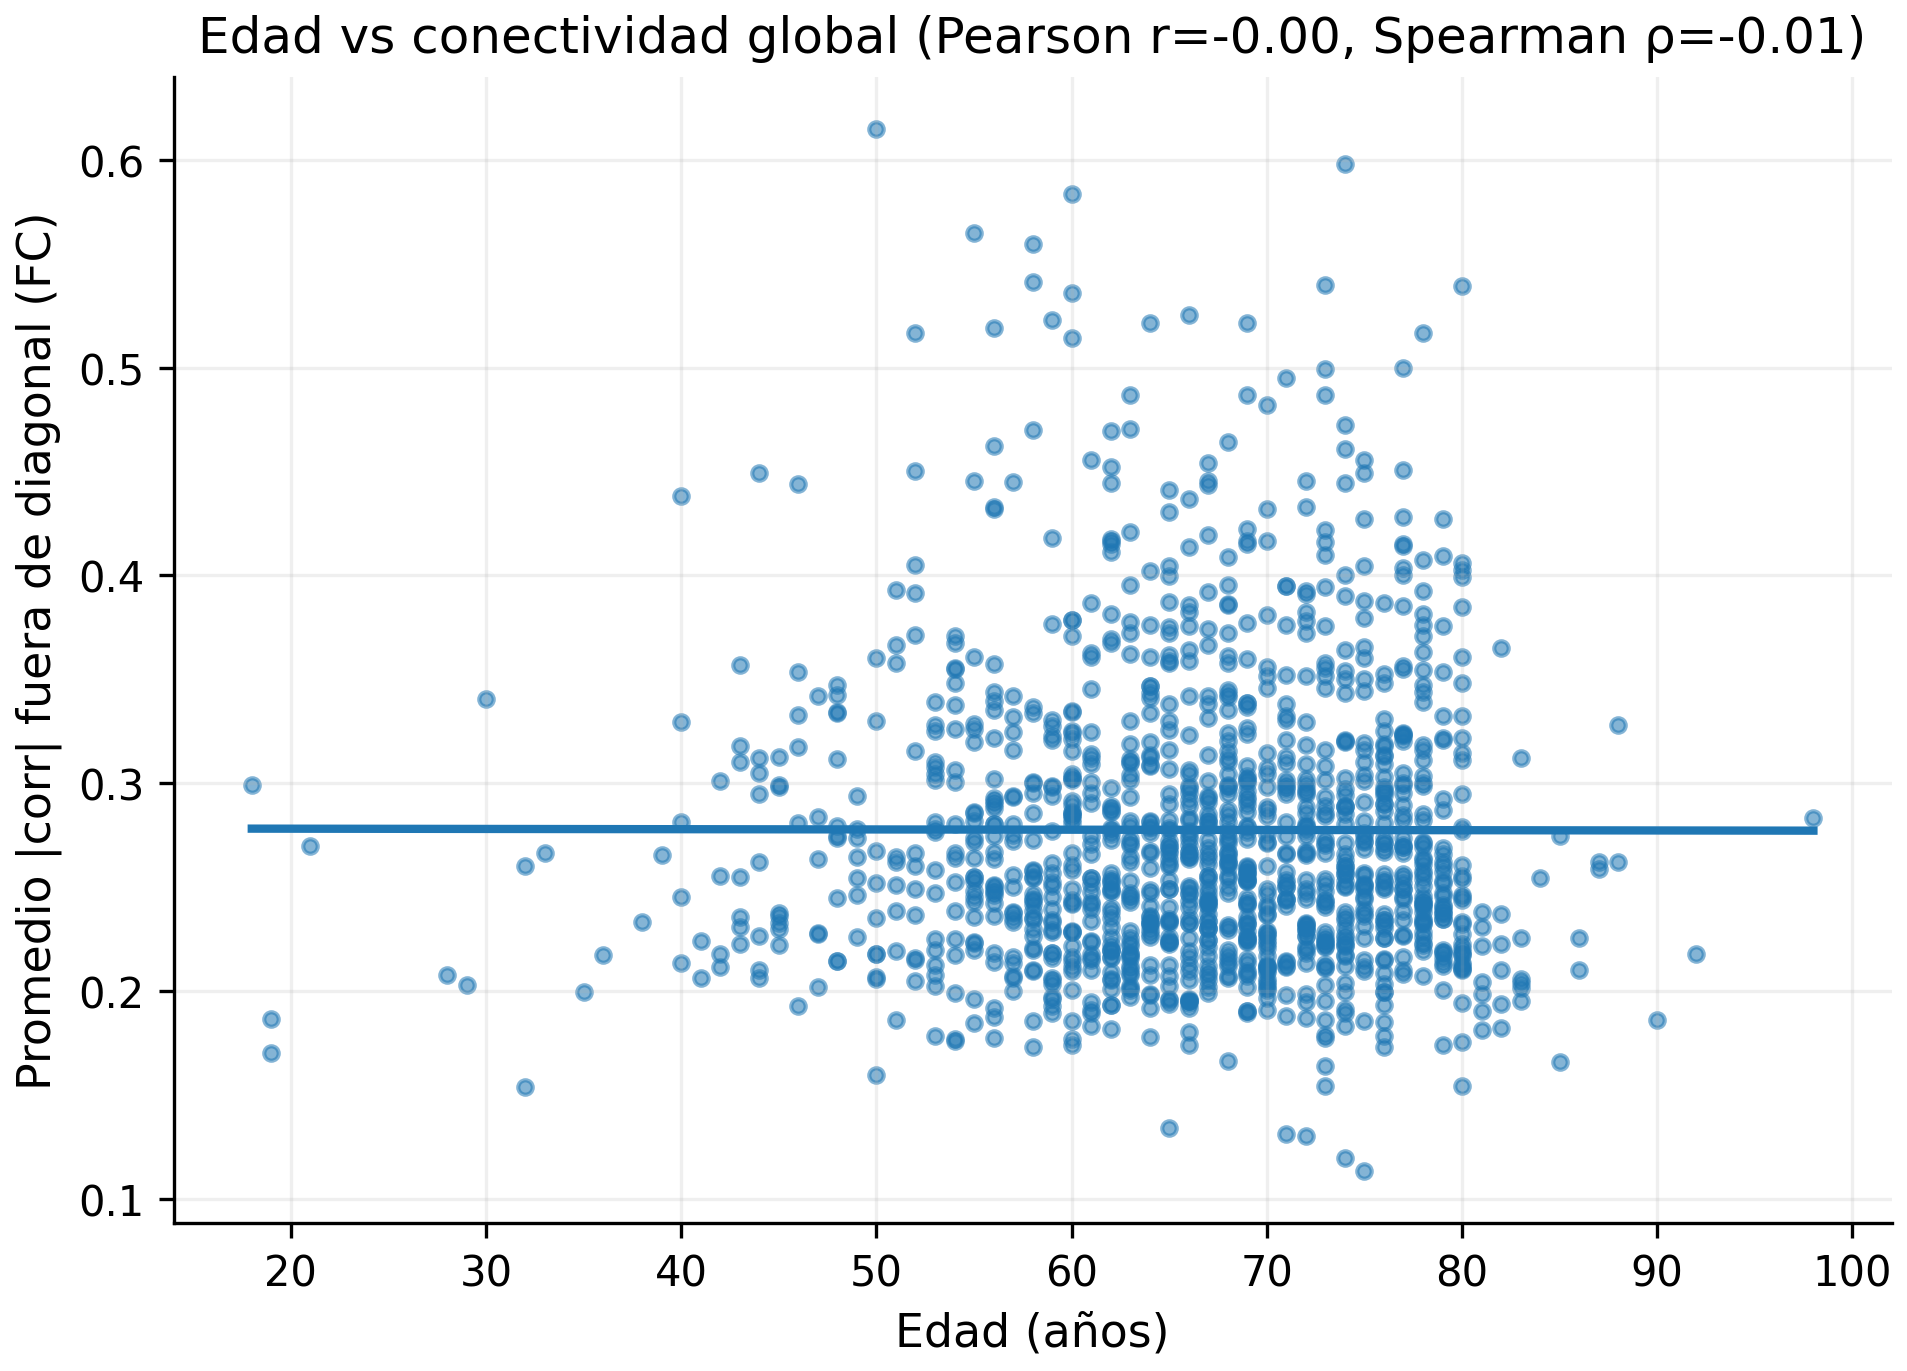
\includegraphics[width=0.80\textwidth]{05_datos_cohorte/images/corr_age_fcmean.png}\\[2pt]
      {\scriptsize FC global vs.\ edad: $r \approx 0$}
    \end{column}
  \end{columns}

  \vspace{0.1cm}
  {\small La FC \textit{global} no correlaciona con la edad, pero la información está en los \highlight{patrones específicos} entre regiones $\rightarrow$ se necesita \textbf{reducción de dimensionalidad}.}
\end{frame}

\begin{frame}{Reducción de dimensionalidad}
  \begin{block}{Necesidad}
    Transformar un espacio de alta dimensión ($p = 6670$) en uno compacto ($k \ll p$), reteniendo la información más relevante para predecir la edad.
  \end{block}

  \vspace{0.3cm}
  \begin{columns}[T]
    \begin{column}{0.46\textwidth}
      \textbf{PCA} (Análisis de Componentes Principales)
      \begin{itemize}
        \item Método \highlight{lineal} clásico
        \item Identifica las direcciones de \textbf{máxima varianza} en los datos
        \item Sin entrenamiento iterativo
        \item Único parámetro: $k$ componentes
      \end{itemize}
    \end{column}
    \begin{column}{0.46\textwidth}
      \textbf{Autoencoders}
      \begin{itemize}
        \item Método \highlight{no lineal}
        \item Red neuronal que aprende a \textbf{comprimir y reconstruir}
        \item Múltiples hiperparámetros
        \item Puede capturar relaciones más complejas
      \end{itemize}
    \end{column}
  \end{columns}

  \vspace{0.3cm}
  \centering
  {\small En este trabajo se comparan ambos enfoques para comprimir las 6670 dimensiones de FC a un espacio de dimensión $k$ (determinado por optimización).}
\end{frame}

\begin{frame}{Autoencoders: comprimir para aprender}
  \begin{columns}[c]
    \begin{column}{0.48\textwidth}
      \begin{itemize}
        \item Red neuronal entrenada de forma \textbf{no supervisada} (no usa etiquetas)
        \item \textbf{Encoder:} entrada $\rightarrow$ representación compacta (espacio latente)
        \item \textbf{Decoder:} representación $\rightarrow$ reconstrucción
        \item El ``cuello de botella'' fuerza a retener solo lo \highlight{más importante}
      \end{itemize}

      \vspace{0.15cm}
      {\small Se entrena minimizando $\mathcal{L}_{\text{rec}}(\mathbf{x}, \tilde{\mathbf{x}})$. Cada dato queda como un \textbf{punto} en el espacio latente.}
    \end{column}
    \begin{column}{0.50\textwidth}
      \centering
      \shorthandoff{>}
      \begin{tikzpicture}[scale=0.75, transform shape,
        >=Stealth, neuron/.style={circle, draw, thick, minimum size=0.42cm},
        input/.style={neuron, fill=teal!20},
        hidden/.style={neuron, fill=blue!15},
        latent/.style={neuron, fill=orange!25},
        conn/.style={-, gray!40, thin},
      ]
        \foreach \i in {1,...,5} {
          \node[input] (in\i) at (0, -\i*0.65 + 1.95) {};
        }
        \node[above=0.1cm of in1, font=\scriptsize\bfseries] {$\mathbf{x}$};
        \node[below=0.1cm of in5, font=\tiny, gray] {$d$ dims};
        \foreach \i in {1,...,3} {
          \node[hidden] (h1\i) at (1.6, -\i*0.65 + 1.3) {};
        }
        \foreach \i in {1,...,2} {
          \node[latent] (z\i) at (3.2, -\i*0.65 + 0.975) {};
        }
        \node[above=0.1cm of z1, font=\scriptsize\bfseries] {$\mathbf{z}$};
        \node[below=0.25cm of z2, font=\tiny, gray] (kdims) {$k$ dims};
        \foreach \i in {1,...,3} {
          \node[hidden] (h2\i) at (4.8, -\i*0.65 + 1.3) {};
        }
        \foreach \i in {1,...,5} {
          \node[input] (out\i) at (6.4, -\i*0.65 + 1.95) {};
        }
        \node[above=0.1cm of out1, font=\scriptsize\bfseries] {$\tilde{\mathbf{x}}$};
        \foreach \i in {1,...,5} {
          \foreach \j in {1,...,3} { \draw[conn] (in\i) -- (h1\j); }}
        \foreach \i in {1,...,3} {
          \foreach \j in {1,...,2} { \draw[conn] (h1\i) -- (z\j); }}
        \foreach \i in {1,...,2} {
          \foreach \j in {1,...,3} { \draw[conn] (z\i) -- (h2\j); }}
        \foreach \i in {1,...,3} {
          \foreach \j in {1,...,5} { \draw[conn] (h2\i) -- (out\j); }}
        \node[font=\tiny, gray] at (0.8, -2.2) {Encoder};
        \node[font=\tiny, gray] at (5.6, -2.2) {Decoder};
        \begin{scope}[shift={(3.2, -2.85)}]
          \draw[->, thick] (-0.7, 0) -- (0.9, 0) node[right, font=\tiny] {$z_1$};
          \draw[->, thick] (0, -0.5) -- (0, 0.8) node[above, font=\tiny] {$z_2$};
          \foreach \px/\py in {-0.5/0.2, -0.3/-0.3, 0.1/0.5, 0.4/-0.2, 0.6/0.3,
                               -0.2/0.4, 0.3/0.05, -0.5/-0.1} {
            \fill[blue!25] (\px, \py) circle (1.2pt);
          }
          \fill[orange!80!red] (0.2, 0.3) circle (2.5pt);
          \draw[-{Stealth[length=1.5mm]}, orange!80!red, semithick] (0.32, 0.39) -- ++(0.2, 0.15)
              node[right, font=\tiny] {$\mathbf{z}_i$};
          \node[below=0.05cm, font=\tiny, gray] at (0, -0.5) {Espacio latente};
        \end{scope}
        \draw[->, dashed, gray] (kdims.south) -- ++(0, -0.25);
      \end{tikzpicture}
      \shorthandon{>}

      \vspace{0.05cm}
      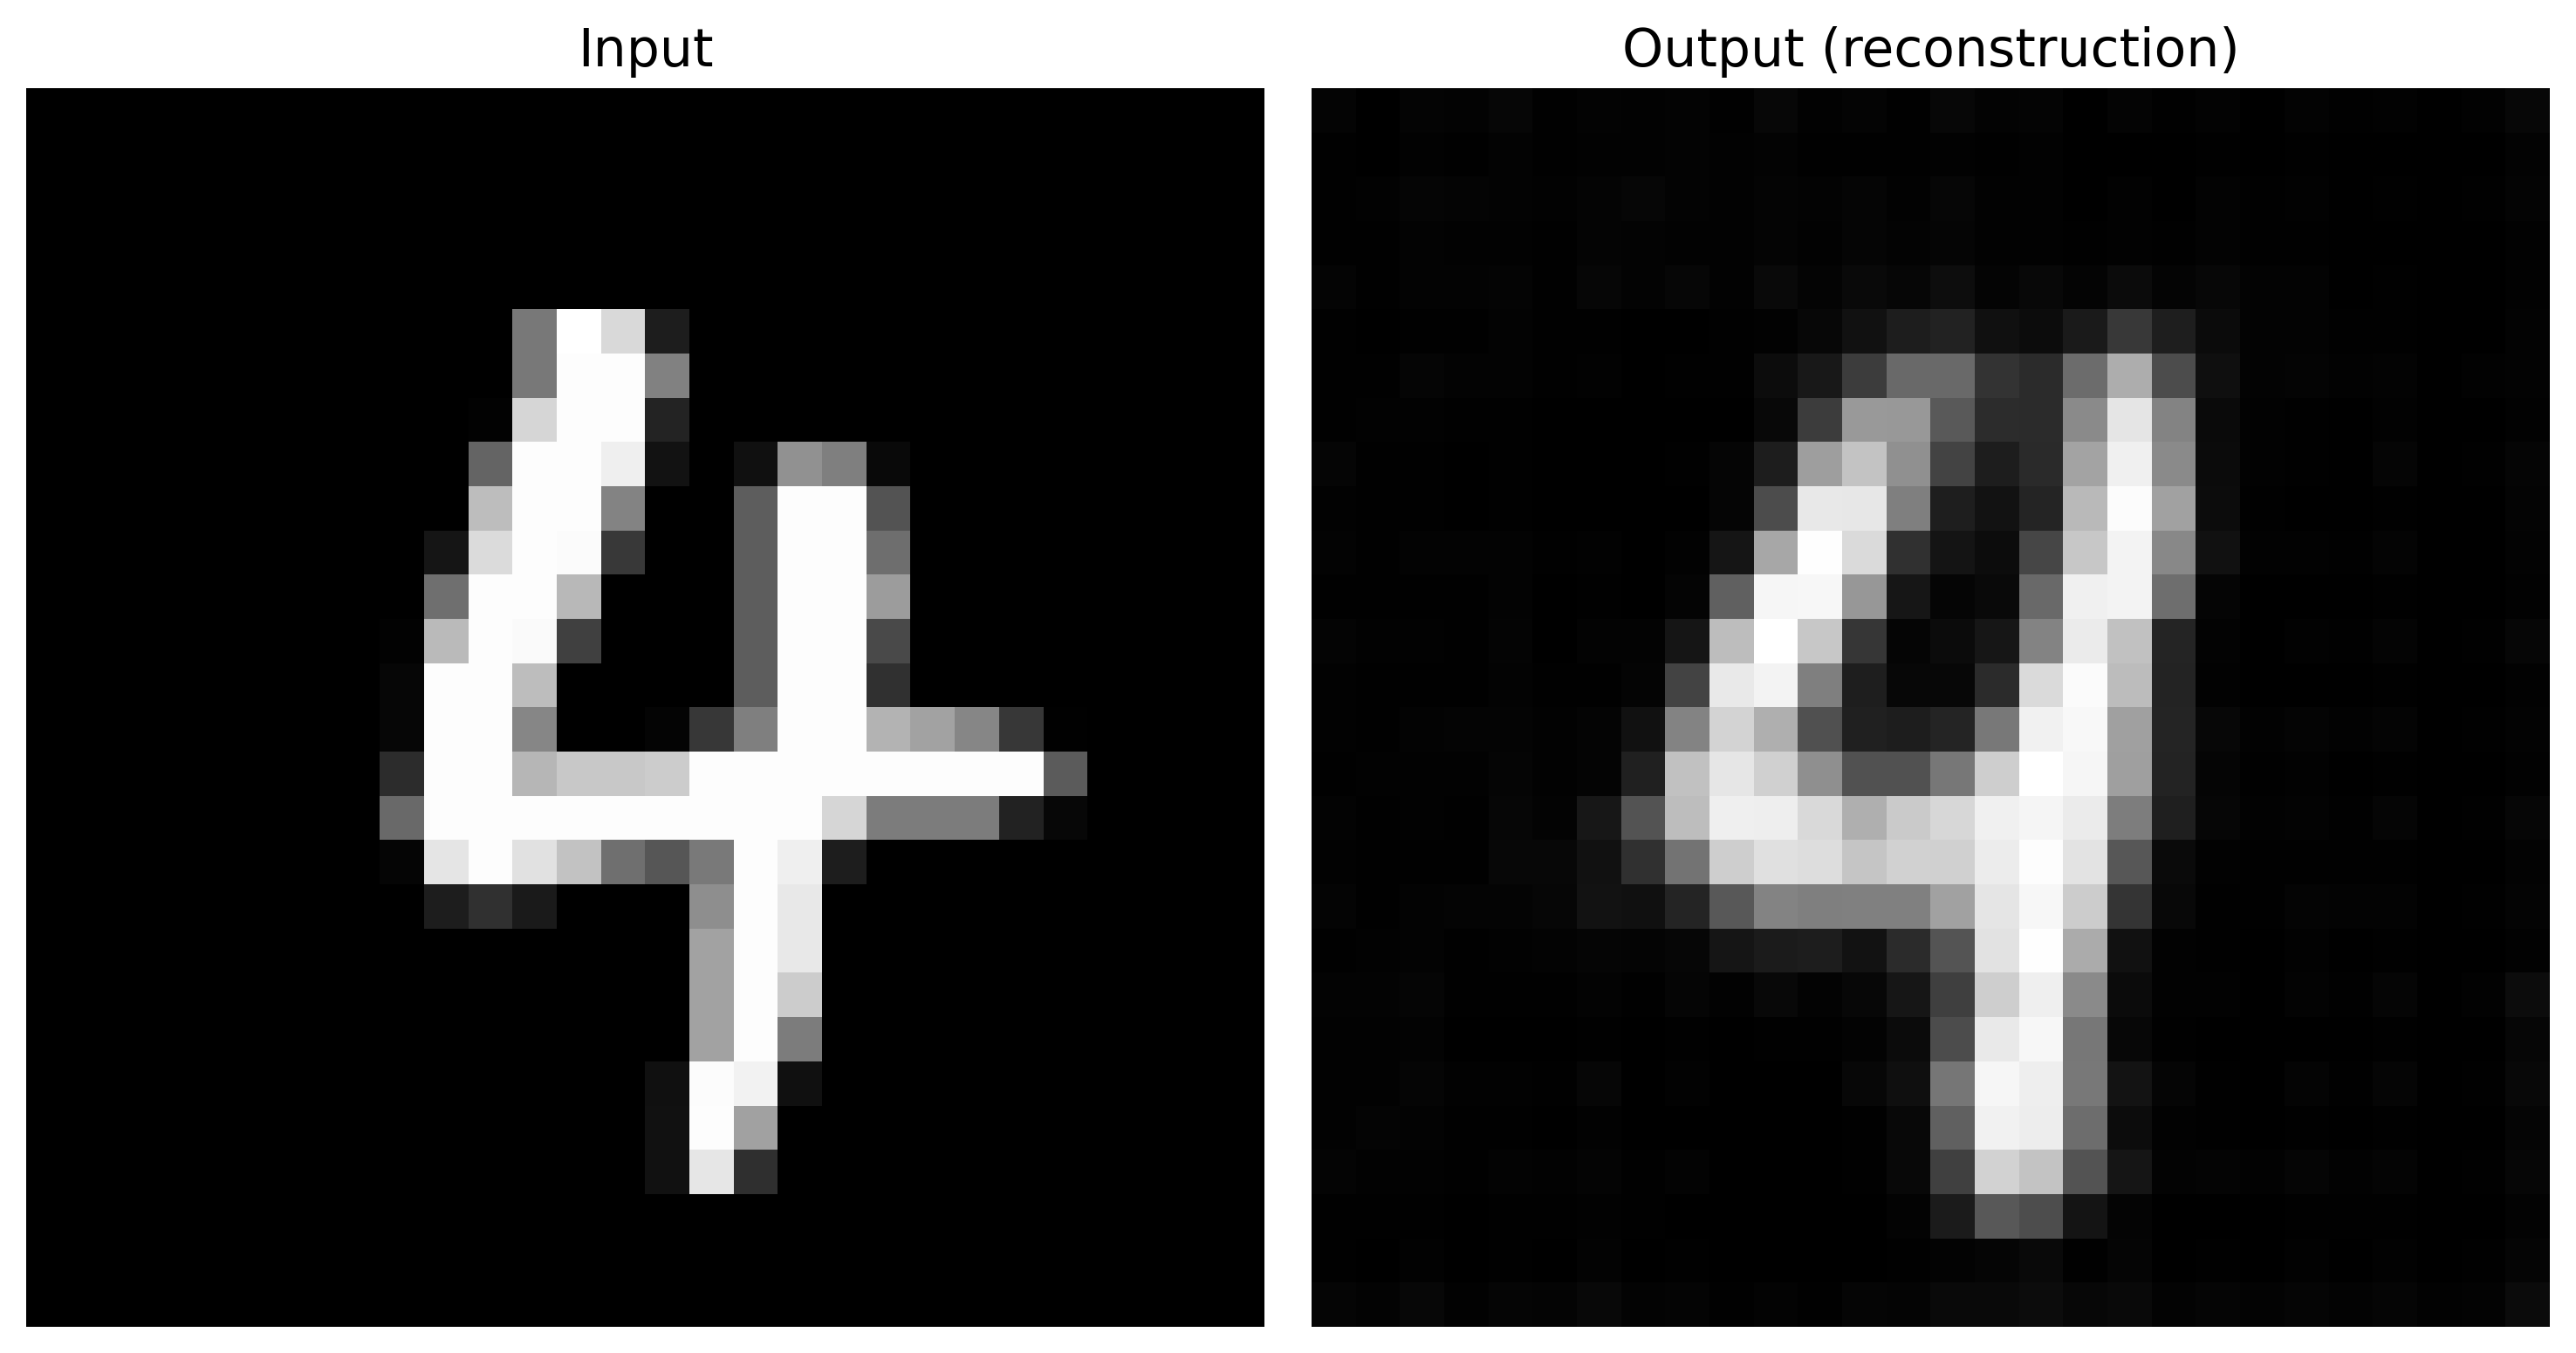
\includegraphics[width=0.36\textwidth]{04_marco_teorico/images/mnist.png}\\[0pt]
      {\scriptsize Ejemplo: dígitos MNIST 28$\times$28}
    \end{column}
  \end{columns}
\end{frame}

\begin{frame}{Autoencoder Variacional (VAE)}
  \begin{columns}[c]
    \begin{column}{0.50\textwidth}
      \textbf{Problema del AE clásico:} el espacio latente puede quedar \textbf{irregular} --- puntos cercanos no necesariamente corresponden a datos similares.

      \vspace{0.2cm}
      \textbf{Solución del VAE:}
      \begin{itemize}
        \item El encoder produce los parámetros de una \highlight{distribución}: $\mu$ y $\sigma$
        \item Se muestrea $z$ con el \textbf{truco de reparametrización}:
      \end{itemize}
      \vspace{-0.2cm}
      \[
        z = \mu + \sigma \odot \epsilon, \quad \epsilon \sim \mathcal{N}(0, I)
      \]

      \vspace{-0.1cm}
      {\small Función de pérdida:}
      \vspace{-0.15cm}
      \[
        \mathcal{L}_{\text{VAE}} = \underbrace{\mathcal{L}_{\text{rec}}}_{\text{\scriptsize fidelidad}} + \underbrace{D_{KL}\big(q(z|x) \,\|\, p(z)\big)}_{\text{\scriptsize regularización}}
      \]
    \end{column}
    \begin{column}{0.48\textwidth}
      \centering
      \shorthandoff{>}
      \begin{tikzpicture}[scale=0.70, transform shape,
        >=Stealth,
        encblock/.style={draw, thick, rounded corners=3pt, minimum height=0.8cm,
                      minimum width=1.3cm, fill=blue!12, font=\small, align=center},
        decblock/.style={draw, thick, rounded corners=3pt, minimum height=0.8cm,
                      minimum width=1.3cm, fill=red!12, font=\small, align=center},
        arr/.style={->, thick},
      ]
        \node (x) {$x$};
        \node[encblock, right=0.5cm of x] (enc) {Encoder\\[-2pt]{\tiny $q(z \mid x)$}};
        \node[draw, thick, circle, minimum size=0.7cm, fill=yellow!15, font=\small, above right=0.5cm and 1cm of enc] (mu) {$\mu$};
        \node[draw, thick, circle, minimum size=0.7cm, fill=orange!15, font=\small, below right=0.5cm and 1cm of enc] (sigma) {$\sigma$};
        \node[draw, thick, circle, minimum size=0.7cm, fill=green!15, font=\small, right=2.8cm of enc] (z) {$z$};
        \node[decblock, right=0.8cm of z] (dec) {Decoder\\[-2pt]{\tiny $p(x \mid z)$}};
        \node[right=0.5cm of dec] (xhat) {$\tilde{x}$};

        \node[below=0.5cm of z, font=\tiny] (eps) {$\epsilon \sim \mathcal{N}(0, I)$};

        \draw[arr] (x) -- (enc);
        \draw[arr] (enc) |- (mu);
        \draw[arr] (enc) |- (sigma);
        \draw[arr] (mu) -- (z);
        \draw[arr] (sigma) -- (z);
        \draw[arr, dashed] (eps) -- (z);
        \draw[arr] (z) -- (dec);
        \draw[arr] (dec) -- (xhat);

        \node[above=0.05cm of z, font=\tiny\itshape] {$z = \mu + \sigma \odot \epsilon$};
      \end{tikzpicture}
      \shorthandon{>}

      \vspace{0.2cm}
      {\scriptsize El espacio latente queda \textbf{continuo} y \textbf{regularizado}: puntos cercanos corresponden a datos similares.}
    \end{column}
  \end{columns}
\end{frame}

\begin{frame}{$\beta$-VAE: controlando el balance}
  \textbf{Extensión del VAE} que agrega un hiperparámetro $\beta$ para ponderar explícitamente la regularización:

  \[
    \mathcal{L}_{\beta\text{-VAE}} = \mathcal{L}_{\text{rec}}(x, \tilde{x}) + \beta \cdot D_{KL}\big(q(z|x) \,\|\, p(z)\big)
  \]

  \begin{columns}[T]
    \begin{column}{0.46\textwidth}
      \begin{block}{$\beta > 1$}
        Mayor regularización\\
        Espacio latente más ordenado\\
        Pero pierde información
      \end{block}
    \end{column}
    \begin{column}{0.46\textwidth}
      \begin{block}{$\beta < 1$}
        \highlight{Preserva información}\\de las matrices FC\\
        Prioriza la reconstrucción
      \end{block}
    \end{column}
  \end{columns}

  \vspace{0.15cm}
  {\small
  \begin{itemize}\setlength{\itemsep}{1pt}
    \item $\beta = 1 \rightarrow$ VAE estándar. Valores óptimos por \textbf{optimización automática}
    \item \textbf{Warmup:} $\beta$ crece desde 0 en las primeras épocas para evitar el \textit{colapso posterior}
    \item $\mathcal{L}_{\text{rec}}$ = MAE, más robusto que MSE ante valores atípicos
  \end{itemize}}
\end{frame}

\begin{frame}{De árboles de decisión a XGBoost}
  \begin{columns}[c]
    \begin{column}{0.52\textwidth}
      {\small \textbf{Árbol de decisión:} divide el espacio de features en regiones
      mediante reglas si/no. Un solo árbol \highlight{sobreajusta}.}

      \vspace{0.15cm}
      {\small \textbf{Gradient Boosting:} muchos árboles \highlight{secuenciales};
      cada uno corrige los \textbf{residuos} del anterior.
      $\hat{y} = \sum_t f_t(x)$}

      \vspace{0.15cm}
      {\small \textbf{XGBoost} --- implementación optimizada:}
      \vspace{-0.1cm}
      {\small
      \begin{itemize}\setlength{\itemsep}{1pt}
        \item \highlight{Regularización} contra sobreajuste
        \item Referencia en \textbf{datos tabulares}
        \item \highlight{Importancia de features} directa (Gain)
      \end{itemize}}

      \vspace{0.05cm}
      {\footnotesize \textbf{En este trabajo:} recibe embeddings FC + T1w y predice la edad. HP optimizados con Optuna.}
    \end{column}
    \begin{column}{0.45\textwidth}
      \centering
      \shorthandoff{>}
      \begin{tikzpicture}[scale=0.65, transform shape,
        tree/.style={draw, rounded corners, minimum width=1.6cm, minimum height=0.55cm, fill=unclight, font=\small},
        arr/.style={->, thick, uncblue}
      ]
        \node[tree] (t1) at (0,0) {Árbol 1};
        \node[tree] (t2) at (0,-1.3) {Árbol 2};
        \node[tree] (t3) at (0,-2.6) {Árbol 3};
        \node[font=\small] (dots) at (0,-3.6) {$\vdots$};
        \node[tree] (tn) at (0,-4.5) {Árbol $N$};

        \node[font=\tiny, right=0.3cm of t1] (r1) {residuos};
        \node[font=\tiny, right=0.3cm of t2] (r2) {residuos};

        \draw[arr] (t1) -- (t2);
        \draw[arr] (t2) -- (t3);
        \draw[arr] (t3) -- (dots);
        \draw[arr] (dots) -- (tn);

        \draw[->, dashed, gray] (r1) to[bend left=20] (t2);
        \draw[->, dashed, gray] (r2) to[bend left=20] (t3);

        \node[draw, rounded corners, fill=uncaccent!15, minimum width=2cm, font=\small, right=1.5cm of t3] (sum) {$\hat{y} = \sum_t f_t$};
        \draw[->, thick, uncblue] (tn.east) -- ++(0.4,0) |- (sum);
      \end{tikzpicture}
      \shorthandon{>}
    \end{column}
  \end{columns}
\end{frame}

\begin{frame}{Validación: partición holdout y $K$-Fold}
  \begin{columns}[c]
    \begin{column}{0.48\textwidth}
      \textbf{Partición holdout:}
      \begin{itemize}
        \item Datos divididos en \textbf{train}, \textbf{validación} y \textbf{test}
        \item El test se reserva para evaluación final
        \item Garantiza métricas no sesgadas
      \end{itemize}

      \vspace{0.3cm}
      \textbf{Validación cruzada $K$-Fold:}
      \begin{itemize}
        \item Los datos de train se dividen en $K$ subconjuntos
        \item En cada iteración, 1 fold valida y $K{-}1$ entrenan
        \item El resultado es el \textbf{promedio} de las $K$ evaluaciones
      \end{itemize}
    \end{column}
    \begin{column}{0.48\textwidth}
      \centering
      \shorthandoff{>}
      \begin{tikzpicture}[scale=0.85, transform shape,
        fold/.style={draw, minimum width=1.2cm, minimum height=0.5cm, font=\tiny},
      ]
        \node[font=\small\bfseries] at (3.2, 1.2) {5-Fold CV};

        \foreach \row in {1,...,5} {
          \node[font=\tiny] at (-0.3, -\row*0.7 + 0.7) {It.\ \row};
          \foreach \col in {1,...,5} {
            \pgfmathtruncatemacro{\isval}{\col==\row ? 1 : 0}
            \ifnum\isval=1
              \node[fold, fill=uncaccent!30] at (\col*1.1, -\row*0.7 + 0.7) {Val};
            \else
              \node[fold, fill=unclight] at (\col*1.1, -\row*0.7 + 0.7) {Train};
            \fi
          }
        }
      \end{tikzpicture}
      \shorthandon{>}

      \vspace{0.2cm}
      {\scriptsize Cada observación es validada exactamente una vez.}
    \end{column}
  \end{columns}
\end{frame}

\begin{frame}{Métricas de regresión}
  {\small Para evaluar qué tan bien un modelo predice una variable continua (la edad):}

  \vspace{0.2cm}
  \begin{columns}[T]
    \begin{column}{0.48\textwidth}
      \begin{block}{MAE (Error absoluto medio)}
        \[
          \text{MAE} = \frac{1}{n} \sum_{i=1}^{n} |y_i - \hat{y}_i|
        \]
        {\scriptsize Error promedio en años. Métrica principal.}
      \end{block}

      \vspace{0.2cm}
      \begin{block}{RMSE}
        \[
          \text{RMSE} = \sqrt{\frac{1}{n} \sum_{i=1}^{n} (y_i - \hat{y}_i)^2}
        \]
        {\scriptsize Penaliza errores grandes.}
      \end{block}
    \end{column}
    \begin{column}{0.48\textwidth}
      \begin{block}{$R^2$ (Coeficiente de determinación)}
        \[
          R^2 = 1 - \frac{\sum (y_i - \hat{y}_i)^2}{\sum (y_i - \bar{y})^2}
        \]
        {\scriptsize Proporción de varianza explicada.\\$R^2 = 1$: perfecto; $R^2 = 0$: predice la media.}
      \end{block}

      \vspace{0.2cm}
      \begin{block}{Pearson $r$}
        {\scriptsize Correlación lineal entre $y$ e $\hat{y}$. Complementa al $R^2$.}
      \end{block}
    \end{column}
  \end{columns}
\end{frame}

\begin{frame}{Optimización de hiperparámetros}
  \begin{itemize}
    \item Los hiperparámetros (learning rate, profundidad, $\beta$, dim.\ latente, \ldots) \textbf{no se aprenden} durante el entrenamiento, se fijan antes
    \item Su elección tiene un impacto significativo en el rendimiento
  \end{itemize}

  \vspace{0.3cm}
  \begin{columns}[T]
    \begin{column}{0.30\textwidth}
      \begin{block}{\small Grid Search}
        {\scriptsize Evalúa todas las combinaciones de una grilla predefinida.\\Costoso si hay muchos parámetros.}
      \end{block}
    \end{column}
    \begin{column}{0.30\textwidth}
      \begin{block}{\small Random Search}
        {\scriptsize Muestrea combinaciones al azar.\\Más eficiente en espacios grandes.}
      \end{block}
    \end{column}
    \begin{column}{0.30\textwidth}
      \begin{block}{\small Optimización Bayesiana}
        {\scriptsize Modela la relación HP $\rightarrow$ métrica y propone configuraciones inteligentes.\\Equilibra exploración y explotación.}
      \end{block}
    \end{column}
  \end{columns}

  \vspace{0.3cm}
  \begin{block}{En este trabajo: Optuna (TPE)}
    Framework de optimización bayesiana usado para ambos modelos ($\beta$-VAE y XGBoost).\\
    Se evalúa cada configuración con \textbf{validación cruzada 5-Fold}.
  \end{block}
\end{frame}


\section{Antecedentes}

\begin{frame}{Antecedentes en la literatura}
  \begin{columns}[T]
    \begin{column}{0.48\textwidth}
      \textbf{Solo MRI estructural:}
      \begin{itemize}
        \item Franke (2010): RVM + PCA, MAE 5,0
        \item Cole (2017): 3D CNN, MAE 4,2
        \item Bashyam (2020): 2D CNN, MAE $\sim$3,7
        \item Kim (2025): DenseNet, MAE 2,7
      \end{itemize}

      \vspace{0.3cm}
      \textbf{Solo conectividad funcional:}
      \begin{itemize}
        \item Gao (2023): GNN + AAL, MAE 5,9
      \end{itemize}
    \end{column}
    \begin{column}{0.48\textwidth}
      \textbf{Multimodales:}
      \begin{itemize}
        \item Liem (2017): stacking, MAE 4,3
        \item Dufumier (2024): M-AVAE, MAE 2,8
      \end{itemize}

      \vspace{0.3cm}
      \textbf{Poblaciones latinoamericanas:}
      \begin{itemize}
        \item Moguilner (2024): GCN + RedLaT
        \item BrainLat (2023): primer dataset multimodal LAC
      \end{itemize}
    \end{column}
  \end{columns}

  \vspace{0.3cm}
  \centering
  {\small \textbf{Tendencia general:} más datos $\rightarrow$ menor error. Multimodal $\geq$ unimodal.}
\end{frame}

\begin{frame}{Posicionamiento de este trabajo}
  \centering
  {\footnotesize
  \begin{tabular}{llcr}
    \toprule
    \textbf{Trabajo} & \textbf{Modalidad / Modelo} & $\boldsymbol{N}$ & \textbf{MAE} \\
    \midrule
    Franke et al. (2010) & T1w (GM) / RVM + PCA & 650 & 5,00 \\
    Cole et al. (2017) & T1w / 3D CNN & 2\,001 & 4,16 \\
    Liem et al. (2017) & T1w+FC / Stacking & 2\,354 & 4,29 \\
    Bashyam et al. (2020) & T1w / 2D CNN & 14\,468 & $\sim$3,7 \\
    Peng et al. (2021) & T1w / SFCN & UK Biobank & $<$3 \\
    Gao et al. (2023) & FC / GNN & 471 & 5,92 \\
    Dufumier et al. (2024) & T1w+FC / M-AVAE & 5\,330 & 2,77 \\
    Kim et al. (2025) & T1w / DenseNet & 8\,681 & 2,73 \\
    \midrule
    \rowcolor{unclight}
    \textbf{Presente trabajo} & \textbf{FC+T1w / $\beta$-VAE+XGB} & \textbf{1\,245} & \textbf{5,62} \\
    \bottomrule
  \end{tabular}}

  \vspace{0.3cm}
  \begin{itemize}
    \item Más datos $\rightarrow$ menor error. Nuestro $N = 1245$ es modesto
    \item $\beta$-VAE y predictor \textbf{separados} (a diferencia de M-AVAE) $\rightarrow$ permite ablaciones
    \item \highlight{Cohorte latinoamericana} — subrepresentada en la literatura
  \end{itemize}
\end{frame}


\section{Datos y cohorte}

\begin{frame}{La cohorte: RedLaT}
  \begin{block}{Red Latinoamericana de Investigación en Neurodegeneración}
    Datos clínicos y de neuroimagen de múltiples centros de América Latina. Cohorte con marcada heterogeneidad socioeconómica, cultural y de protocolos de adquisición.
  \end{block}

  \vspace{0.2cm}
  \textbf{Fuentes de datos integradas:}
  \begin{enumerate}
    \item \textbf{Matrices FC:} $116 \times 116$ de fMRI en reposo
    \item \textbf{Volúmenes T1w:} 116 valores regionales de materia gris
    \item \textbf{Metadatos clínicos:} edad, sexo, diagnóstico (CN, AD, FTD)
    \item \textbf{Variables demográficas:} años de educación, sitio de adquisición, marca de escáner (disponibles para $\sim$75\% de la cohorte)
  \end{enumerate}

  \vspace{0.3cm}
  \centering
  \shorthandoff{>}
  \begin{tikzpicture}[
    box/.style={draw, rounded corners, align=center, text width=2.2cm,
                minimum height=0.8cm, font=\footnotesize},
    arr/.style={-{Stealth[length=2.5mm]}, thick, uncblue}
  ]
    \node[box, fill=unclight] (fc) {FC\\$N{=}1365$};
    \node[box, fill=unclight, right=0.8cm of fc] (meta) {Metadatos\\$N{=}1327$};
    \node[box, fill=unclight, right=0.8cm of meta] (t1) {T1w\\$N{=}2748$};
    \node[box, fill=uncaccent!15, right=0.8cm of t1, text width=2.8cm] (final)
      {\textbf{Cohorte final}\\$\boldsymbol{N{=}1245}$};
    \draw[arr] (fc) -- (meta);
    \draw[arr] (meta) -- (t1);
    \draw[arr] (t1) -- (final);
  \end{tikzpicture}
  \shorthandon{>}
\end{frame}

\begin{frame}{Descripción demográfica}
  \begin{columns}[T]
    \begin{column}{0.48\textwidth}
      \centering
      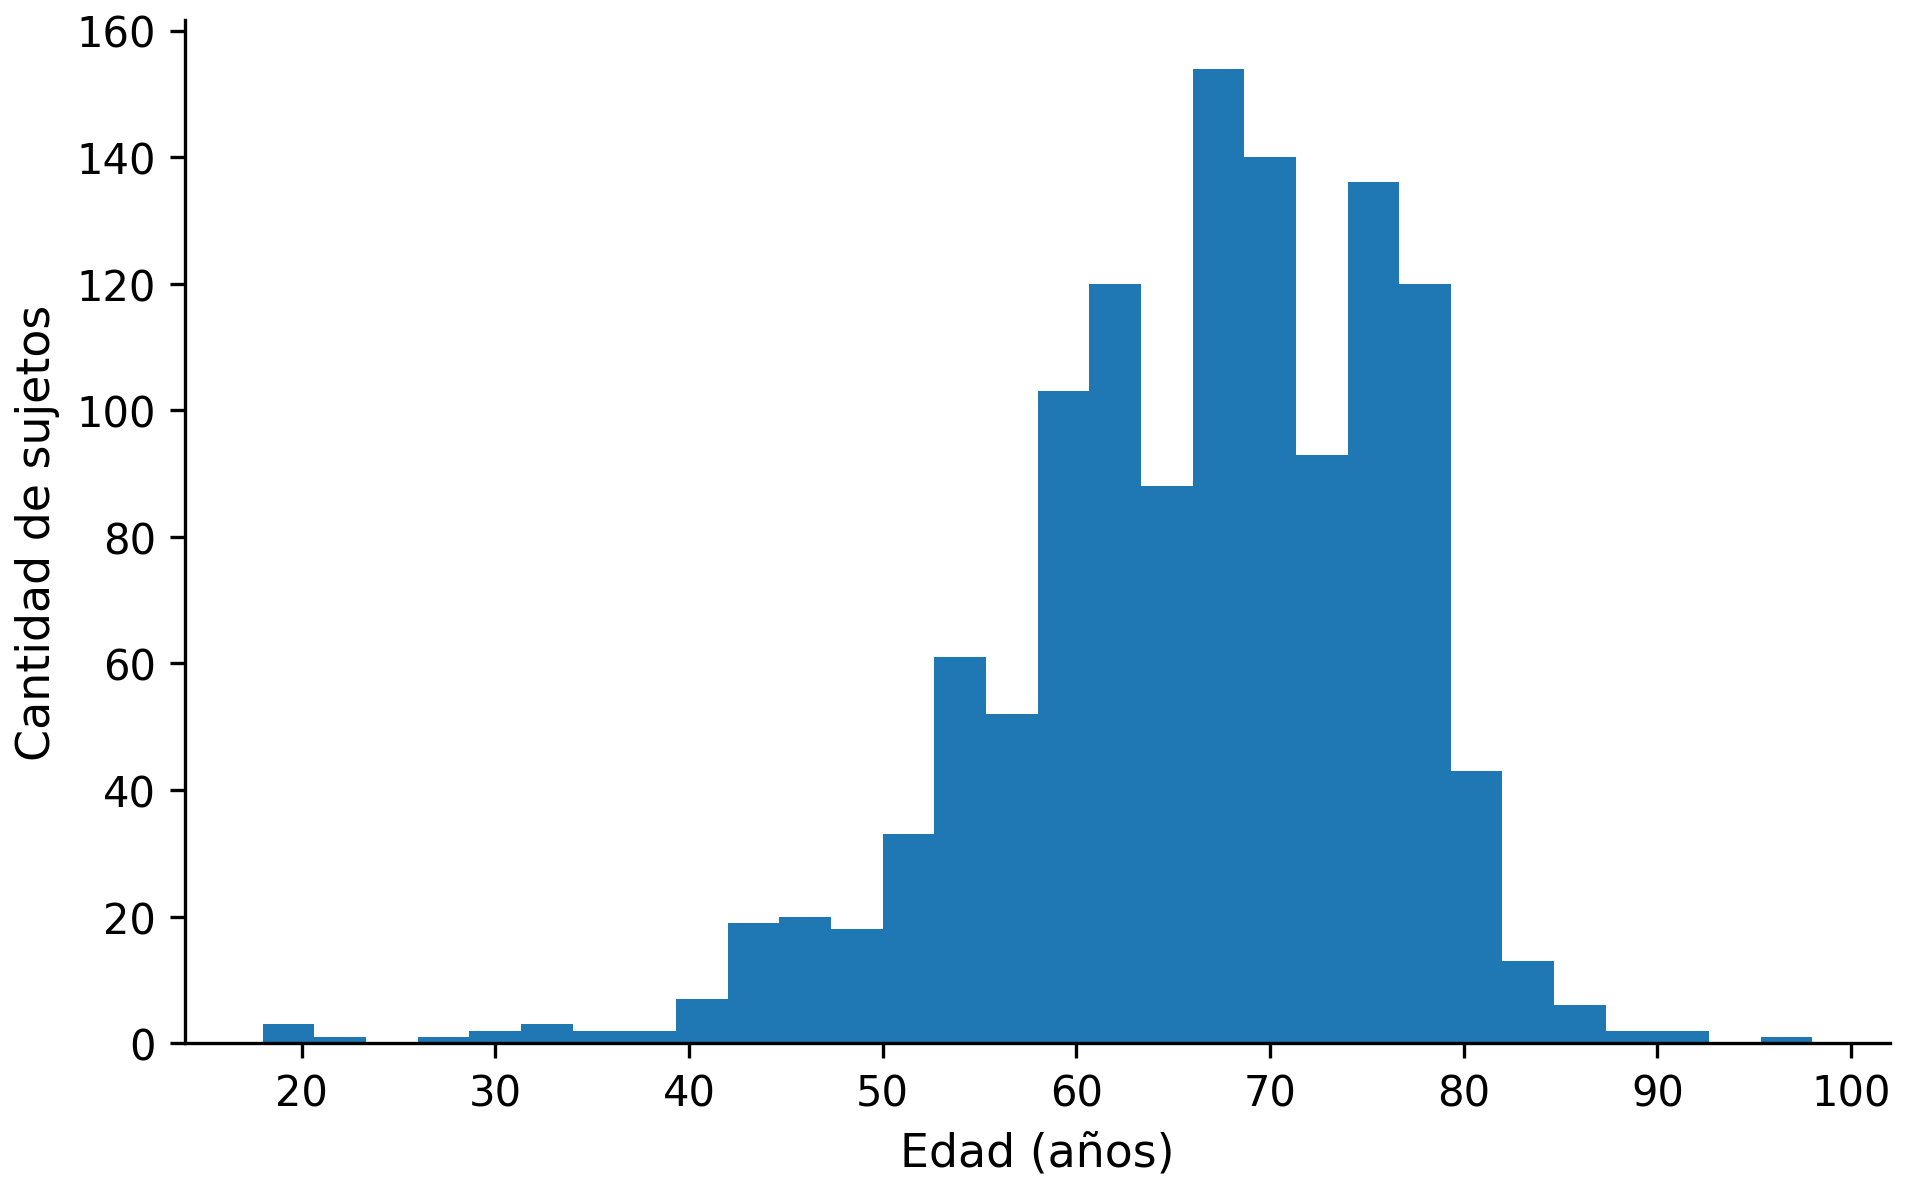
\includegraphics[width=\textwidth]{05_datos_cohorte/images/age_hist.png}\\[2pt]
      {\scriptsize Distribución de edades (rango 18--98)}
    \end{column}
    \begin{column}{0.48\textwidth}
      \centering
      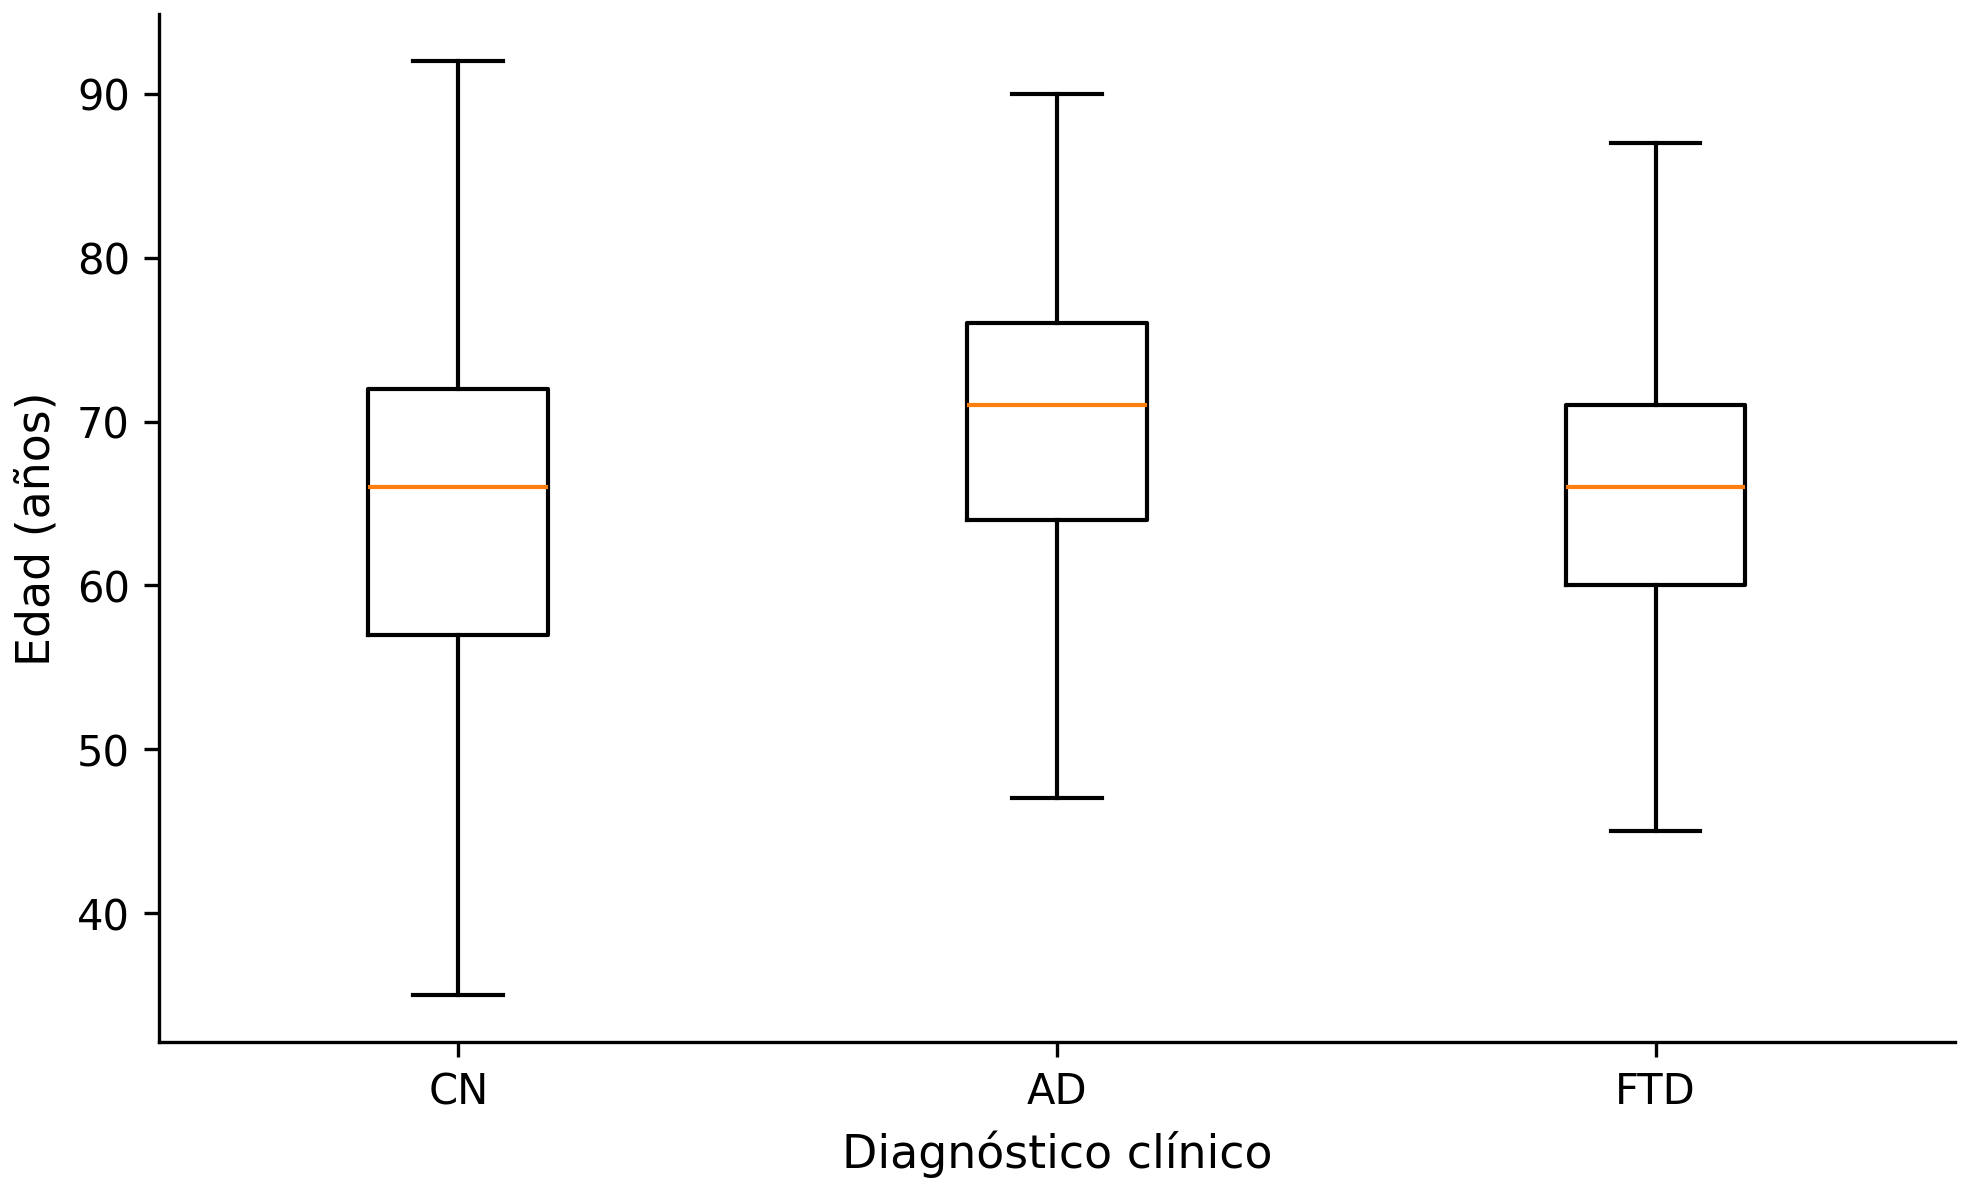
\includegraphics[width=\textwidth]{05_datos_cohorte/images/age_by_diag_box.png}\\[2pt]
      {\scriptsize Edad por diagnóstico clínico}
    \end{column}
  \end{columns}

  \vspace{0.3cm}
  \centering
  {\small
  \begin{tabular}{lrrr}
    \toprule
    & \textbf{CN} & \textbf{AD} & \textbf{FTD} \\
    \midrule
    $N$ & 526 & 422 & 297 \\
    Edad (media $\pm$ DE) & $64 \pm 15$ & $72 \pm 10$ & $66 \pm 10$ \\
    \bottomrule
  \end{tabular}}
\end{frame}


\section{Metodología}

\begin{frame}{Pipeline general}
  \centering
  \shorthandoff{>}
  \begin{tikzpicture}[scale=0.75, transform shape,
    node distance=0.5cm and 0.8cm,
    block/.style={rectangle, draw, rounded corners, text width=2.6cm,
                  minimum height=0.65cm, align=center, font=\small},
    data/.style={rectangle, draw, dashed, rounded corners, text width=2.4cm,
                 minimum height=0.55cm, align=center, font=\small, fill=gray!10},
    arrow/.style={-{Stealth[length=2.5mm]}, thick, uncblue}
  ]
    \node[data] (fc) {Matrices FC\\$(116 \times 116)$};
    \node[data, right=2.2cm of fc] (t1w) {Volúmenes T1w\\(116 regiones)};

    \node[block, below=of fc, fill=unclight] (preproc) {Fisher $z$ + vectorización\\(6670 dims)};
    \node[block, below=of preproc, fill=unclight] (vae) {$\beta$-VAE Encoder};
    \node[data, below=of vae] (emb) {Embeddings $\mu$ (64 dims)};
    \node[block, below=0.6cm of emb, xshift=1.1cm, fill=uncaccent!15] (concat) {Concatenación (180 dims)};
    \node[block, below=of concat, fill=unclight] (xgb) {XGBoost};
    \node[data, below=of xgb] (pred) {Edad predicha $\hat{y}$};

    \draw[arrow] (fc) -- (preproc);
    \draw[arrow] (preproc) -- (vae);
    \draw[arrow] (vae) -- (emb);
    \draw[arrow] (emb) -- (concat);
    \draw[arrow] (t1w) |- (concat);
    \draw[arrow] (concat) -- (xgb);
    \draw[arrow] (xgb) -- (pred);
  \end{tikzpicture}
  \shorthandon{>}
\end{frame}

\begin{frame}{División de los datos}
  \centering
  \shorthandoff{>}
  \begin{tikzpicture}[
    box/.style={draw, rounded corners, text width=2.8cm, align=center,
                minimum height=0.9cm, font=\small},
    arr/.style={-{Stealth[length=2.5mm]}, thick, uncblue}
  ]
    \node[box, fill=unclight] (all) {Cohorte\\$N = 1245$};
    \node[box, fill=unclight, below left=1cm and 0.2cm of all] (tv) {Trainval (90\%)\\$n = 1120$};
    \node[box, fill=uncaccent!15, below right=1cm and 0.2cm of all] (test) {Test (10\%)\\$n = 125$};
    \node[box, fill=unclight!50, below=1cm of tv, text width=3.2cm] (cv) {5-Fold CV\\hiperparámetros};
    \draw[arr] (all) -- (tv);
    \draw[arr] (all) -- (test);
    \draw[arr] (tv) -- (cv);
  \end{tikzpicture}
  \shorthandon{>}

  \vspace{0.4cm}
  \begin{itemize}
    \item Partición \textbf{estratificada} por sexo y diagnóstico
    \item El test set \textbf{nunca} se usa para decisiones de diseño
    \item Los mismos 5 folds en todas las etapas $\rightarrow$ comparaciones justas
  \end{itemize}
\end{frame}

\begin{frame}{Optimización en dos etapas}
  \begin{columns}[T]
    \begin{column}{0.46\textwidth}
      \begin{alertblock}{\scriptsize Enfoque tradicional}
        {\scriptsize Optimizar $\beta$-VAE para reconstruir bien
        $\rightarrow$ Podría capturar ruido irrelevante}
      \end{alertblock}
    \end{column}
    \begin{column}{0.46\textwidth}
      \begin{block}{\scriptsize Nuestro enfoque (\textit{downstream})}
        {\scriptsize Optimizar $\beta$-VAE según predicción de edad
        $\rightarrow$ Representaciones orientadas al envejecimiento}
      \end{block}
    \end{column}
  \end{columns}

  \vspace{0.1cm}
  \centering
  \shorthandoff{>}
  \begin{tikzpicture}[scale=0.60, transform shape,
    stage/.style={draw, thick, rounded corners=5pt, minimum width=3.8cm,
                  minimum height=1.2cm, align=center, font=\small},
    optstep/.style={draw, rounded corners=2pt, minimum width=2.8cm,
                 minimum height=0.5cm, align=center, font=\scriptsize, fill=unclight},
    frozen/.style={optstep, dashed, fill=gray!15},
    arr/.style={-{Stealth[length=2.5mm]}, thick, uncblue},
    lbl/.style={font=\tiny, gray}
  ]
    \node[stage, fill=uncblue!15] (e1) at (0, 0) {\textbf{Etapa 1}\\Optuna $\beta$-VAE};
    \node[stage, fill=uncblue!15] (e2) at (5.5, 0) {\textbf{Etapa 2}\\Optuna XGBoost};
    \node[stage, fill=uncaccent!15] (e3) at (11, 0) {\textbf{Etapa 3}\\Modelo final};

    \node[optstep] (vae1) at (0, -2) {Entrenar $\beta$-VAE\\con HP propuestos};
    \node[frozen] (xgb1) at (0, -3.5) {XGBoost\\(params fijos)};
    \node[lbl] at (0, -4.3) {$\times$ 70 trials, 5-fold CV};

    \node[frozen] (vae2) at (5.5, -2) {$\beta$-VAE fijo\\(mejor de Etapa 1)};
    \node[optstep] (xgb2) at (5.5, -3.5) {Entrenar XGBoost\\con HP propuestos};
    \node[lbl] at (5.5, -4.3) {$\times$ 100 trials, 5-fold CV};

    \node[optstep] (vae3) at (11, -2) {$\beta$-VAE final\\(todo trainval)};
    \node[optstep] (xgb3) at (11, -3.5) {XGBoost final\\(todo trainval)};
    \node[lbl] at (11, -4.3) {Evaluar en test holdout};

    \draw[arr] (e1) -- (e2);
    \draw[arr] (e2) -- (e3);
    \draw[arr] (e1) -- (vae1);
    \draw[arr] (vae1) -- (xgb1);
    \draw[arr] (e2) -- (vae2);
    \draw[arr] (vae2) -- (xgb2);
    \draw[arr] (e3) -- (vae3);
    \draw[arr] (vae3) -- (xgb3);
  \end{tikzpicture}
  \shorthandon{>}

  \vspace{0.15cm}
  {\small
  \begin{itemize}\setlength{\itemsep}{1pt}
    \item Componentes \textbf{congelados} (borde discontinuo) no se optimizan en esa etapa
    \item Estructura \textbf{modular}: permite intercambiar el regresor sin reentrenar el $\beta$-VAE
  \end{itemize}}
\end{frame}

\begin{frame}{Configuración óptima del $\beta$-VAE (Optuna)}
  \begin{block}{Resultado de la optimización downstream}
    {\small Optuna determinó $\beta = 0{,}057$ ($\ll 1$): el modelo prioriza \highlight{preservar la información} de las matrices FC.}
  \end{block}

  \vspace{0.2cm}
  \begin{columns}[T]
    \begin{column}{0.48\textwidth}
      {\small \textbf{Arquitectura resultante:}}
      \begin{itemize}
        \item Encoder: $6670 \to 512 \to (\mu, \sigma) \in \mathbb{R}^{64}$
        \item Decoder simétrico: $64 \to 512 \to 6670$
        \item Activación: ELU
        \item Layer Normalization
        \item Dropout: 0,037
        \item Regularización L2: $2{,}9 \times 10^{-7}$
      \end{itemize}
    \end{column}
    \begin{column}{0.48\textwidth}
      {\small \textbf{Entrenamiento:}}
      \begin{itemize}
        \item $\mathcal{L}_{\text{rec}}$ = MAE
        \item Warmup: 73 épocas
        \item Embeddings usados: $\mu$ (determinístico)
        \item Dimensión latente: 64
      \end{itemize}

      \vspace{0.2cm}
      {\scriptsize Vector final por sujeto: 64 (FC) + 116 (T1w) = \highlight{180 features}}
    \end{column}
  \end{columns}
\end{frame}

\begin{frame}{Estrategia de evaluación}
  Se diseñaron \textbf{siete análisis complementarios}:

  \vspace{0.3cm}
  \begin{enumerate}
    \item \textbf{Modelo principal:} $\beta$-VAE + T1w $\rightarrow$ XGBoost en test holdout

    \vspace{0.1cm}
    \item \textbf{Ablaciones:} 7 combinaciones de features (FC, T1w, sexo, diagnóstico)

    \vspace{0.1cm}
    \item \textbf{PCA vs.\ $\beta$-VAE:} misma dimensionalidad (64), mismo regresor

    \vspace{0.1cm}
    \item \textbf{FC crudo vs.\ $\beta$-VAE:} 6786 features crudos vs.\ 180 comprimidos

    \vspace{0.1cm}
    \item \textbf{Comparación de regresores:} Ridge, SVR y XGBoost optimizados

    \vspace{0.1cm}
    \item \textbf{Variables demográficas:} impacto de educación y sitio sobre la brain age gap y como features predictivas

    \vspace{0.1cm}
    \item \textbf{Entrenamiento solo CN:} explorar viabilidad como biomarcador de envejecimiento acelerado
  \end{enumerate}
\end{frame}


\begin{frame}{Pipeline: resumen animado}
  \centering
  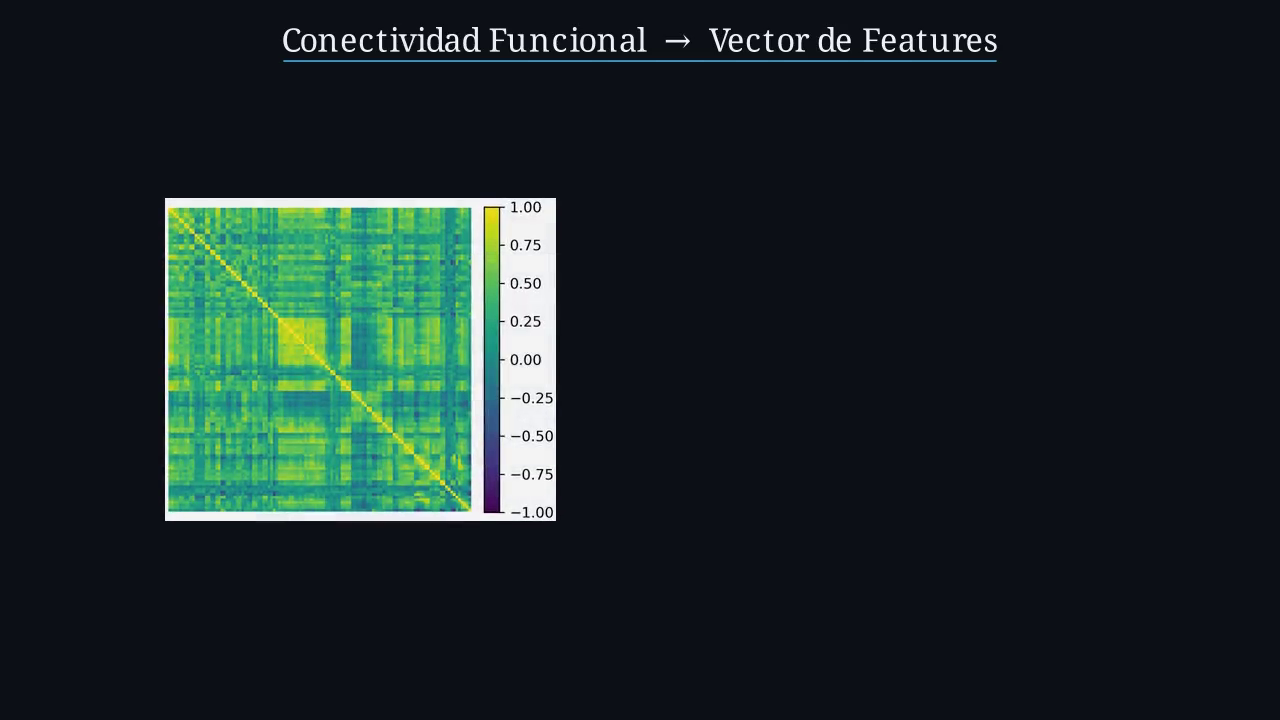
\includegraphics[width=0.75\linewidth, height=0.62\textheight, keepaspectratio]{07_pipeline_animado/pipeline_poster.png}

  \vspace{0.15cm}
  {\small Recorrido completo: FC $\to$ $\beta$-VAE $\to$ fusión multimodal $\to$ XGBoost.}

\end{frame}


\section{Resultados}

\begin{frame}{Reconstrucción del $\beta$-VAE}
  \begin{columns}[c]
    \begin{column}{0.38\textwidth}
      \centering
      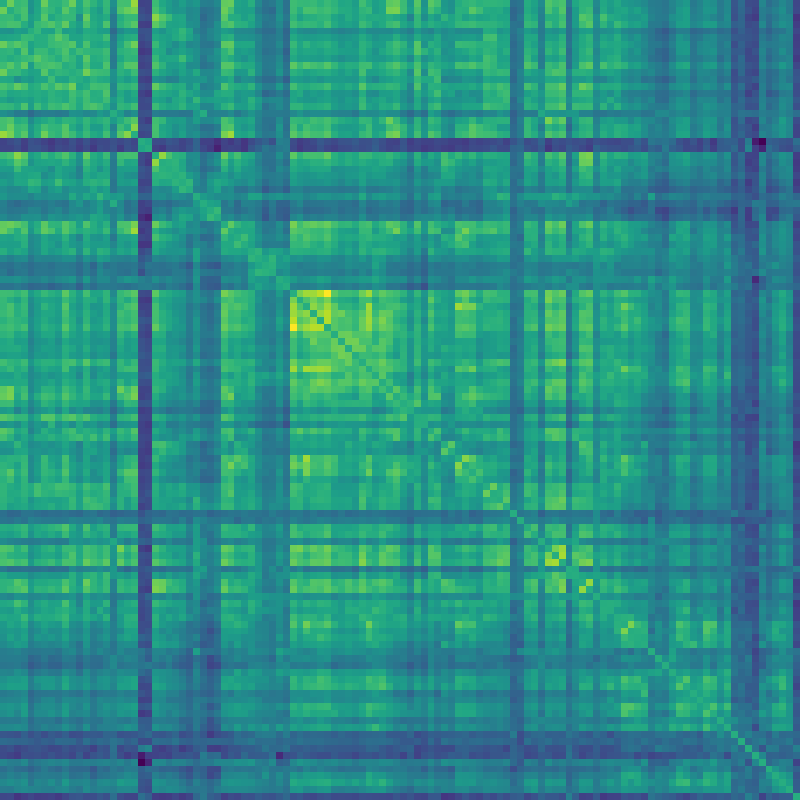
\includegraphics[width=\textwidth]{06_resultados_discusion/images/vae_recon_original_best.png}\\[3pt]
      {\small \textbf{FC original}}
    \end{column}
    \begin{column}{0.38\textwidth}
      \centering
      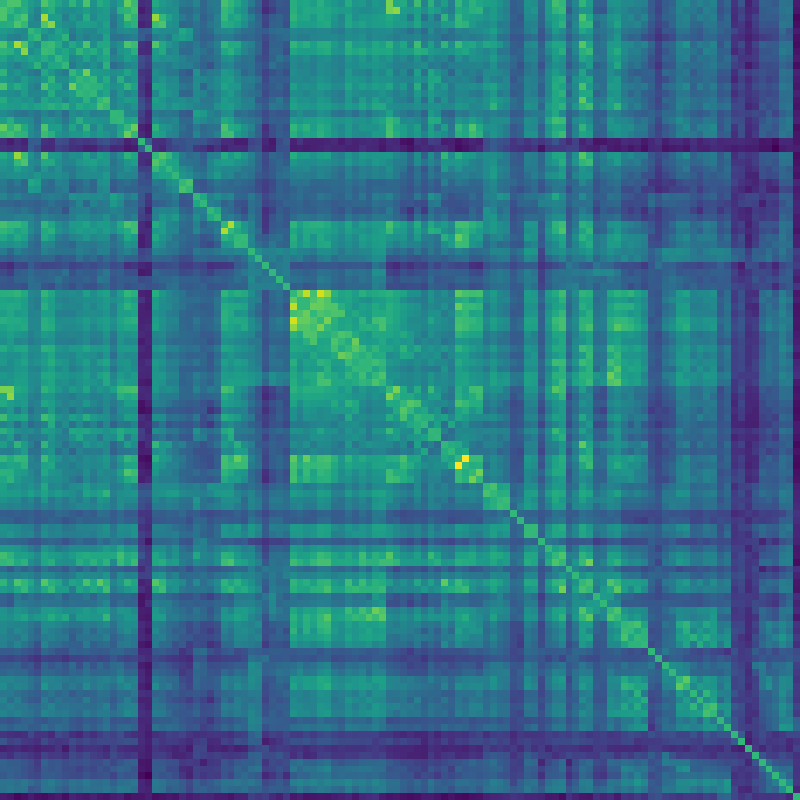
\includegraphics[width=\textwidth]{06_resultados_discusion/images/vae_recon_reconstructed_best.png}\\[3pt]
      {\small \textbf{FC reconstruida} ($r = 0{,}884$)}
    \end{column}
    \begin{column}{0.22\textwidth}
      {\scriptsize
      \begin{tabular}{lr}
        \toprule
        \textbf{Métrica} & \textbf{Val.} \\
        \midrule
        Pearson & 0,79 \\
        Coseno & 0,87 \\
        MAE & 0,124 \\
        \bottomrule
      \end{tabular}}

      \vspace{0.2cm}
      {\scriptsize \highlight{99\%} compresión\\$6670 \to 64$ dims}
    \end{column}
  \end{columns}

  \vspace{0.15cm}
  \centering
  {\small Patrones globales de conectividad preservados; detalles finos suavizados por la compresión.}
\end{frame}

\begin{frame}{Resultado del modelo principal}
  \begin{columns}[T]
    \begin{column}{0.48\textwidth}
      \centering
      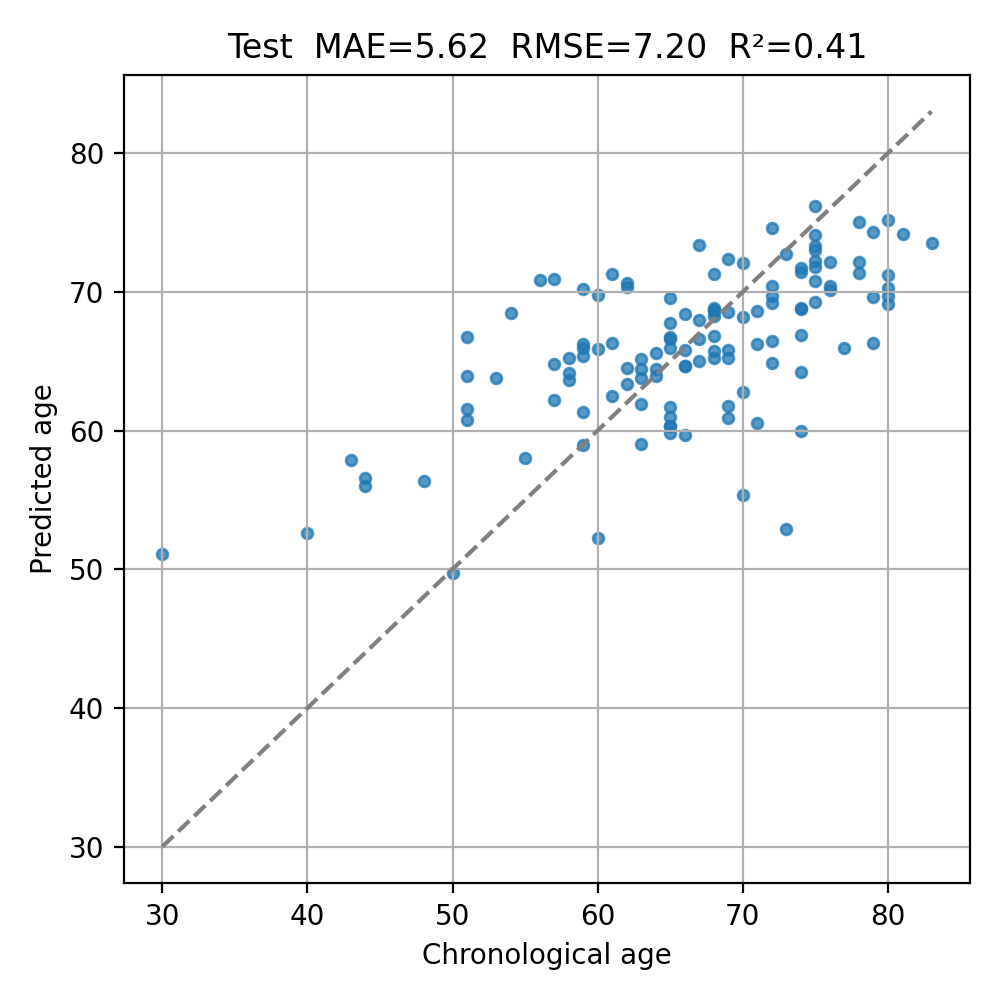
\includegraphics[width=0.92\textwidth]{06_resultados_discusion/images/xgb_scatter.png}\\[2pt]
      {\scriptsize Edad predicha vs.\ edad real ($n = 125$)}
    \end{column}
    \begin{column}{0.48\textwidth}
      \begin{block}{Métricas en test}
        \centering
        {\small
        \begin{tabular}{lr}
          \toprule
          \textbf{MAE} & \highlight{5,62 años} \\
          RMSE & 7,20 años \\
          $R^2$ & 0,411 \\
          Pearson & 0,644 \\
          \bottomrule
        \end{tabular}}
      \end{block}

      \vspace{0.1cm}
      {\small Error promedio de $\sim$5,6 años.\\Comparable con Gao et al.\ (5,92) con cohorte más diversa.}

      \vspace{0.1cm}
      {\scriptsize Mayor dispersión en extremos del rango etario.}
    \end{column}
  \end{columns}
\end{frame}

\begin{frame}{Importancia de features (XGBoost)}
  \begin{columns}[T]
    \begin{column}{0.55\textwidth}
      \centering
      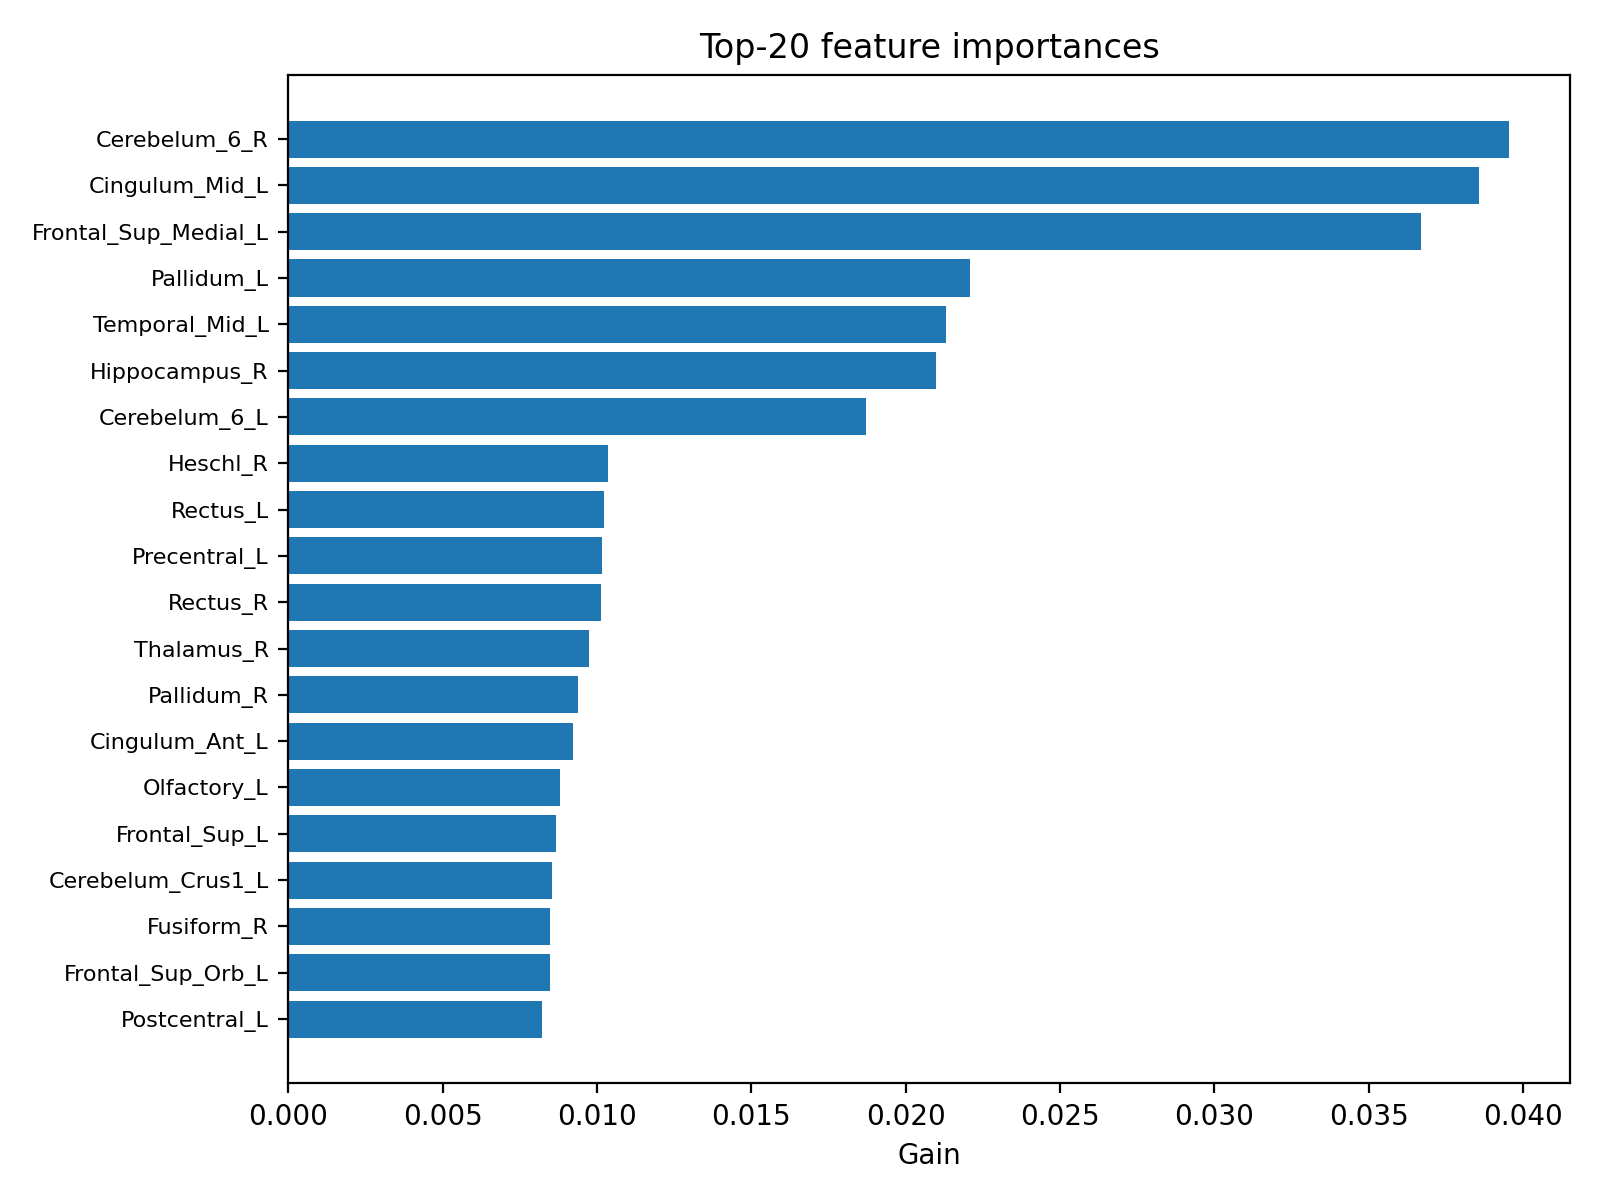
\includegraphics[width=\textwidth]{06_resultados_discusion/images/xgb_importance_top20.png}
    \end{column}
    \begin{column}{0.42\textwidth}
      {\small
      Las etiquetas son las regiones del atlas AAL (T1w) que más contribuyen a la predicción. Las que aparecen arriba (cerebelo, cíngulo, frontal, pallidum, temporal, hipocampo, tálamo) suelen reportarse en la literatura como estructuras con cambios asociados a la edad.

      \vspace{0.2cm}
      XGBoost da estas importancias de forma directa (Gain en los árboles). Con otros regresores, interpretar la contribución individual de cada feature resulta más complejo.
      }
    \end{column}
  \end{columns}
\end{frame}

\begin{frame}{Estudio de ablaciones}
  \centering
  {\footnotesize
  \begin{tabular}{lrrrr}
    \toprule
    \textbf{Features} & \textbf{MAE} & \textbf{RMSE} & $\boldsymbol{R^2}$ & $\boldsymbol{r}$ \\
    \midrule
    Solo T1w (116) & 5,89 & 7,48 & 0,366 & 0,606 \\
    T1w + sexo (117) & 5,88 & 7,44 & 0,372 & 0,612 \\
    Solo $\beta$-VAE (64) & 7,01 & 9,12 & 0,056 & 0,284 \\
    $\beta$-VAE + sexo (65) & 7,06 & 9,18 & 0,044 & 0,268 \\
    \rowcolor{unclight}
    \textbf{$\beta$-VAE + T1w (180)} & \textbf{5,62} & \textbf{7,20} & \textbf{0,411} & \textbf{0,644} \\
    $\beta$-VAE + T1w + sexo (181) & 5,70 & 7,34 & 0,389 & 0,626 \\
    $\beta$-VAE + T1w + sexo + dx (182) & 5,64 & 7,17 & 0,416 & 0,648 \\
    \bottomrule
  \end{tabular}}

  \vspace{0.15cm}
  \begin{columns}[T]
    \begin{column}{0.48\textwidth}
      \begin{block}{Conclusiones}
        \begin{itemize}
          \item FC + T1w \highlight{$>$} cualquiera sola
          \item $\beta$-VAE solo: $R^2 = 0{,}056$ (insuficiente)
          \item Sexo y diagnóstico no mejoran
        \end{itemize}
      \end{block}
    \end{column}
    \begin{column}{0.48\textwidth}
      \centering
      {\small Modalidades \highlight{complementarias}:\\
      agregar FC reduce MAE en 0,27 años\\respecto a T1w sola}
    \end{column}
  \end{columns}
\end{frame}

\begin{frame}{PCA vs.\ $\beta$-VAE: ¿importa la no linealidad?}
  \centering
  {\small
  \begin{tabular}{lrrrr}
    \toprule
    \textbf{Método} & \textbf{MAE} & \textbf{RMSE} & $\boldsymbol{R^2}$ & $\boldsymbol{r}$ \\
    \midrule
    PCA + T1w & 5,61 & 7,08 & 0,431 & 0,661 \\
    $\beta$-VAE + T1w & 5,62 & 7,20 & 0,411 & 0,644 \\
    \bottomrule
  \end{tabular}}

  \vspace{0.5cm}
  \begin{columns}[T]
    \begin{column}{0.46\textwidth}
      \begin{block}{Resultado clave}
        \centering
        Rendimiento \highlight{prácticamente idéntico}\\[4pt]
        {\small Diferencias $< 0{,}02$ en todas las métricas}
      \end{block}
    \end{column}
    \begin{column}{0.46\textwidth}
      \vspace{0.2cm}
      XGBoost puede extraer patrones no lineales aun desde PCA\\[6pt]
      Lo clave es la \highlight{reducción} ($6670 \rightarrow 64$),\\no si es lineal o no lineal\\[6pt]
      {\scriptsize \textit{Nota:} Optuna exploró solo 70 de un espacio combinatorio vasto para el $\beta$-VAE}
    \end{column}
  \end{columns}
\end{frame}

\begin{frame}{FC crudo vs.\ $\beta$-VAE: ¿es necesaria la reducción?}
  {\small XGBoost optimizado \textbf{independientemente} con Optuna para cada configuración:}

  \vspace{0.2cm}
  \centering
  {\small
  \begin{tabular}{lrrrrr}
    \toprule
    \textbf{Método} & \textbf{Features} & \textbf{MAE} & \textbf{RMSE} & $\boldsymbol{R^2}$ & $\boldsymbol{r}$ \\
    \midrule
    FC crudo + T1w & 6786 & 6,00 & 7,55 & 0,354 & 0,601 \\
    \rowcolor{unclight}
    \textbf{$\beta$-VAE + T1w} & \textbf{180} & \textbf{5,62} & \textbf{7,20} & \textbf{0,411} & \textbf{0,644} \\
    \bottomrule
  \end{tabular}}

  \vspace{0.4cm}
  \begin{columns}[T]
    \begin{column}{0.46\textwidth}
      \begin{block}{Resultado clave}
        \centering
        \highlight{97,3\%} menos features\\y \highlight{0,38 años} mejor MAE\\[4pt]
        {\small $R^2$: $+$16\% relativo}
      \end{block}
    \end{column}
    \begin{column}{0.46\textwidth}
      \vspace{0.2cm}
      Optuna para FC crudo: árboles poco profundos, solo 10\% de features por árbol\\[6pt]
      $\rightarrow$ $\beta$-VAE hace esta selección de forma más \highlight{sistemática y efectiva}
    \end{column}
  \end{columns}
\end{frame}

\begin{frame}{Comparación de regresores}
  {\small Todos optimizados con Optuna (100 trials, 5-fold CV), mismos features ($\beta$-VAE + T1w):}

  \vspace{0.2cm}
  \centering
  {\small
  \begin{tabular}{lrrrr}
    \toprule
    \textbf{Regresor} & \textbf{MAE} & \textbf{RMSE} & $\boldsymbol{R^2}$ & $\boldsymbol{r}$ \\
    \midrule
    Ridge & 5,75 & 7,25 & 0,403 & 0,639 \\
    SVR (RBF) & 5,65 & 7,02 & 0,441 & 0,664 \\
    \rowcolor{unclight}
    \textbf{XGBoost} & \textbf{5,62} & 7,20 & 0,411 & 0,644 \\
    \bottomrule
  \end{tabular}}

  \vspace{0.4cm}
  \begin{block}{Hallazgo}
    Tres familias muy distintas (lineal, kernel, árboles) $\rightarrow$ resultados \highlight{prácticamente iguales}
  \end{block}

  \vspace{0.2cm}
  \textbf{Implicación:} la \highlight{calidad de la representación} aprendida es el factor determinante, no la elección del regresor.
\end{frame}

\begin{frame}{Entrenamiento solo en controles sanos}
  \begin{block}{Idea}
    Entrenar solo con sujetos sanos ($n = 473$) y evaluar la brain age gap en \textbf{todos} los pacientes clínicos (no vistos durante el entrenamiento).
  \end{block}

  \vspace{0.3cm}
  \centering
  {\small
  \begin{tabular}{lrrrrr}
    \toprule
    \textbf{Grupo} & $\boldsymbol{n}$ & \textbf{MAE} & $\boldsymbol{R^2}$ & \textbf{Gap} \\
    \midrule
    CN (test)   & 53  & 6,03 & 0,504    & $-0{,}42$ \\
    AD (todos)  & 422 & 7,36 & $-0,170$ & $-1{,}86$ \\
    FTD (todos) & 297 & 6,93 & $-0,153$ & $+1{,}84$ \\
    \bottomrule
  \end{tabular}}

  \vspace{0.3cm}
  \begin{columns}[T]
    \begin{column}{0.46\textwidth}
      \begin{alertblock}{Problema}
        {\small MAE 6,03 en CN $>$ 5,62 (mixto)\\
        $R^2$ negativo en AD y FTD\\
        Gap inconsistente: $-1{,}86$ en AD, $+1{,}84$ en FTD}
      \end{alertblock}
    \end{column}
    \begin{column}{0.46\textwidth}
      \begin{block}{Conclusión}
        {\small Optuna dedicada para CN confirma: limitación es el tamaño muestral, no los hiperparámetros. Se necesitan $N > 2000$ CN.}
      \end{block}
    \end{column}
  \end{columns}
\end{frame}


\begin{frame}{Variables demográficas: educación}
  \begin{block}{Variable: \texttt{cog\_ed} — años de educación formal (disponible 74,9\%)}
    {\small Indicador del nivel socioeconómico. Se analizó su correlación con la brain age gap por grupo diagnóstico.}
  \end{block}

  \vspace{0.3cm}
  \centering
  {\small
  \begin{tabular}{lrrl}
    \toprule
    \textbf{Grupo} & $\boldsymbol{r}$ & $\boldsymbol{p}$ & \textbf{Interpretación} \\
    \midrule
    CN  & $-0{,}067$ & $0{,}19$ & tendencia negativa, no significativa \\
    AD  & $+0{,}165$ & $0{,}002$ & significativa ($\uparrow$ educación $\rightarrow$ gap más alta) \\
    FTD & $\approx 0$ & $0{,}98$ & sin correlación \\
    \bottomrule
  \end{tabular}}

  \vspace{0.35cm}
  \begin{columns}[T]
    \begin{column}{0.46\textwidth}
      \begin{block}{CN}
        {\small Dirección negativa $\rightarrow$ educación actúa como \textbf{factor neuroprotector} (reserva cognitiva). Señal débil con $n = 473$.}
      \end{block}
    \end{column}
    \begin{column}{0.46\textwidth}
      \begin{block}{AD}
        {\small Más educación $\rightarrow$ gap más positiva: diagnóstico tardío en estadios avanzados (\textbf{reserva cognitiva invierte el patrón}).}
      \end{block}
    \end{column}
  \end{columns}
\end{frame}

\begin{frame}{Variables demográficas: sitio y escáner}
  \begin{block}{El sitio de adquisición es el mayor confundidor}
    ANOVA: $F = 8{,}67$,\ $p < 0{,}001$ \quad $\rightarrow$ diferencias significativas entre los 11 centros.
  \end{block}

  \vspace{0.2cm}
  \begin{columns}[T]
    \begin{column}{0.52\textwidth}
      {\small
      \begin{tabular}{lrr}
        \toprule
        \textbf{Sitio} & $\boldsymbol{n}$ & \textbf{Gap media} \\
        \midrule
        Bruno       & 48  & $+4{,}30$ años \\
        Takada      & 89  & $+2{,}82$ \\
        Matallana   & 135 & $+0{,}92$ \\
        Miller      & 400 & $-0{,}20$ \\
        Lopera      & 88  & $-3{,}64$ \\
        \bottomrule
      \end{tabular}}
      \\[4pt]
      {\scriptsize Diferencia máxima $\approx$ 8 años entre sitios.}
    \end{column}
    \begin{column}{0.44\textwidth}
      \textbf{Por marca de escáner:}
      \vspace{0.15cm}
      {\small
      \begin{tabular}{lrr}
        \toprule
        \textbf{Escáner} & $\boldsymbol{n}$ & \textbf{Gap} \\
        \midrule
        Philips  &  47 & $+4{,}33$ \\
        GE       & 289 & $+0{,}95$ \\
        Siemens  & 581 & $-0{,}26$ \\
        \bottomrule
      \end{tabular}}
      \vspace{0.25cm}
      \begin{alertblock}{\small Conclusión}
        {\footnotesize Un modelo con educación, sexo, diagnóstico y sitio explica el \textbf{8\%} de la varianza de la gap; el sitio es el principal contribuyente. Necesario: armonización ComBat.}
      \end{alertblock}
    \end{column}
  \end{columns}
\end{frame}

\begin{frame}{Demográficos como features: optimización con Optuna}
  \begin{block}{Experimento}
    {\small Incluir educación y sitio como features adicionales. El sitio se codifica mediante \textit{one-hot}: una columna binaria por centro (p.~ej.\ \texttt{site\_Miller} = 1 si el sujeto es de Miller, 0 si no). Hiperparámetros de XGBoost optimizados \textbf{independientemente} (Optuna, 100 trials) para cada configuración.}
  \end{block}

  \vspace{0.2cm}
  \centering
  {\small
  \begin{tabular}{lrrrr}
    \toprule
    \textbf{Configuración} & $\boldsymbol{n_{\text{test}}}$ & \textbf{MAE} & $\boldsymbol{R^2}$ & $\boldsymbol{r}$ \\
    \midrule
    $\beta$-VAE + T1w (baseline) & 125 & 5,62 & 0,411 & 0,644 \\
    + educación & 91 & 5,33 & 0,502 & 0,711 \\
    + sitio & 93 & 5,37 & 0,538 & 0,744 \\
    \rowcolor{unclight}
    \textbf{+ educación + sitio} & \textbf{91} & \highlight{5,17} & \textbf{0,523} & \textbf{0,725} \\
    \bottomrule
  \end{tabular}}

  \vspace{0.3cm}
  \begin{columns}[T]
    \begin{column}{0.46\textwidth}
      \begin{block}{Resultado clave}
        {\small MAE \highlight{5,17}: mejor configuración. Mejora de 0,45 años sobre baseline.}
      \end{block}
    \end{column}
    \begin{column}{0.46\textwidth}
      {\small Las features demográficas contienen información predictiva complementaria a la neuroimagen. Ambas fuentes se posicionan entre las top 20 en importancia.}
    \end{column}
  \end{columns}
\end{frame}

\begin{frame}{CN-only + demográficos: hacia un biomarcador}
  \begin{block}{Experimento exploratorio}
    {\small Entrenar solo con 337 CN (que tienen datos demográficos) incluyendo educación y sitio.}
  \end{block}

  \vspace{0.2cm}
  \centering
  {\small
  \begin{tabular}{llrrrr}
    \toprule
    \textbf{Modelo} & \textbf{Grupo} & $\boldsymbol{n}$ & \textbf{MAE} & \textbf{Gap} \\
    \midrule
    CN baseline (337) & CN (test) & 53 & 6,09 & $-0{,}07$ \\
                & AD       & 422 & 6,97 & $+0{,}21$ \\
                & FTD      & 297 & 7,42 & $+4{,}01$ \\
    \midrule
    CN + edu + sitio & CN (test) & 37 & \highlight{5,51} & $+0{,}41$ \\
                     & AD       & 348 & 6,41 & $+0{,}70$ \\
                     & FTD      & 211 & 6,49 & \highlight{$+4{,}11$} \\
    \bottomrule
  \end{tabular}}

  \vspace{0.25cm}
  {\small Gaps \highlight{consistentemente positivas} en AD y FTD $\rightarrow$ dirección esperada en neurodegeneración.\\
  Resultado prometedor: con más datos CN, el pipeline podría funcionar como biomarcador.}
\end{frame}


\section{Discusión y conclusiones}

\begin{frame}{Discusión}
  \begin{itemize}
    \item \textbf{MAE de 5,62} dentro del rango de la literatura para cohortes comparables
    \begin{itemize}
      \item Gao et al.: MAE 5,92 con GNN ($N = 471$)
      \item Franke et al.: MAE 5,00 con RVM ($N = 650$, solo T1w)
    \end{itemize}

    \vspace{0.3cm}
    \item Trabajos con MAE $< 3$ usan cohortes \textbf{mucho mayores} ($N > 5000$)

    \vspace{0.3cm}
    \item Nuestra cohorte \highlight{latinoamericana} tiene mayor heterogeneidad (multi-sitio, multi-país)

    \vspace{0.3cm}
    \item $R^2 = 0{,}41$: queda varianza por explicar $\rightarrow$ margen de mejora

    \vspace{0.3cm}
    \item \highlight{CN-only + demográficos: MAE 5,51} --- mejor que el modelo mixto (5,62) y más comparable con la literatura (entrenan solo con sanos)
  \end{itemize}
\end{frame}

\begin{frame}{Limitaciones}
  \begin{enumerate}
    \item \textbf{Tamaño de la cohorte:} $N = 1245$ es modesto comparado con estudios recientes

    \vspace{0.25cm}
    \item \textbf{Heterogeneidad multi-sitio:} sin armonización entre centros (ComBat)

    \vspace{0.25cm}
    \item \textbf{Resolución del atlas:} AAL 116 regiones es grueso; atlas finos podrían capturar patrones más sutiles

    \vspace{0.25cm}
    \item \textbf{Sin modelos end-to-end:} no se comparó con 3D CNN ni GNN

    \vspace{0.25cm}
    \item \textbf{Exploración del $\beta$-VAE:} solo 70 trials de Optuna sobre un espacio combinatorio vasto; una mejor configuración podría superar a PCA
  \end{enumerate}
\end{frame}

\begin{frame}{Conclusiones}
  \begin{enumerate}
    \item Pipeline multimodal (FC + T1w) con MAE de \highlight{5,62 años}; con educación y sitio: \highlight{MAE 5,17}. CN-only + demográficos: \highlight{MAE 5,51}

    \vspace{0.18cm}
    \item La integración de ambas modalidades mejora la predicción\\$\rightarrow$ las fuentes son \highlight{complementarias}

    \vspace{0.18cm}
    \item $\beta$-VAE $\approx$ PCA con XGBoost optimizado; la \highlight{reducción} es clave: supera a FC crudo (5,62 vs.\ 6,00)

    \vspace{0.18cm}
    \item El \highlight{sitio de adquisición} es el mayor confundidor demográfico ($\sim$8 años de rango); armonización necesaria

    \vspace{0.18cm}
    \item CN-only + demográficos: \highlight{MAE 5,51} (mejor que mixto) con gaps positivas en AD y FTD $\rightarrow$ \highlight{prometedor} como biomarcador

    \vspace{0.18cm}
    \item Evaluado sobre cohorte \highlight{latinoamericana multicéntrica}; resultados relevantes en contexto LAC
  \end{enumerate}
\end{frame}

\begin{frame}{Trabajo futuro}
  \begin{columns}[T]
    \begin{column}{0.48\textwidth}
      \textbf{Datos:}
      \begin{itemize}
        \item Ampliar cohorte (especialmente CN, $N > 2000$)
        \item \textbf{Armonización multi-sitio} (ComBat, NeuroHarmonize)
        \item Atlas de mayor resolución
        \item Más features estructurales (materia blanca, LCR)
        \item Análisis demográfico ampliado (ingresos, ocupación, estatus socioeconómico y edad de inicio ---ao---)
      \end{itemize}
    \end{column}
    \begin{column}{0.48\textwidth}
      \textbf{Modelos:}
      \begin{itemize}
        \item Comparar optimización downstream vs.\ reconstrucción pura
        \item Modelos end-to-end (GNN, 3D CNN)
        \item Datos longitudinales
        \item Otras modalidades (DTI, grosor cortical)
      \end{itemize}
    \end{column}
  \end{columns}
\end{frame}

\begin{frame}{Agradecimientos}
  \vspace{2.5cm}
  \centering
  {\large Agradecimientos}
\end{frame}

\begin{frame}{}
  \vspace{2cm}
  \centering
  {\Huge \textcolor{uncblue}{¡Gracias!}}\\[1cm]
  {\Large ¿Preguntas?}\\[1.2cm]
  {\small
    Nicolás Marcelo Bazán\\
    FaMAF --- Universidad Nacional de Córdoba\\[0.35cm]
    Código: \url{https://github.com/BazanNicolas/Thesis-Computer-Science}
  }
\end{frame}

\end{document}
